%#!platex latex2022.tex
\documentclass{jsarticle}
\usepackage{fancybox,ascmac}
\usepackage{epstopdf}
\usepackage[dvipdfmx]{graphicx}
\usepackage{amsmath,amssymb}
\usepackage{bm}
\usepackage{alltt}
\usepackage{authblk}
\usepackage{fancyhdr}
\usepackage{url}

\topmargin -0.8in
\oddsidemargin -0.3in
\textheight 10in
\textwidth 7in

\pagestyle{fancy}
    \lhead{{\LaTeX 入門}} %ヘッダ左
    %\chead{ヘッダ中央} %ヘッダ中央
    \rhead{2022年4月13日(水) \ 地球惑星物理学演習} %ヘッダ右.コンパイルした日付を表示
    % \lfoot{} %フッタ左
    \cfoot{—\, \thepage \, —} %フッタ中央.ページ番号を表示
    %\rfoot{© 著作権} %フッタ右


\title{\LaTeX 入門}
\author{高田 大成\thanks{固体地球科学講座 田中愛幸研究室 修士1年, Email: takata@eps.s.u-tokyo.ac.jp}}
\date{2022年4月13日(水) \\
\vspace*{2cm}
\begin{flushleft}
\section*{はじめに}
\ \ \ 本郷に進学し、みなさんはこれからレポートなどの文書を作成する機会も益々多
 くなることと思います。特にこの学科にいれば、数式・図を多く含んだ文書を
 作りたくなるでしょう。\\
\ \ \ 今回は、\LaTeX という組版ソフトを紹介します。皆さんの中にはもうすでに使ったことがある方もいらっしゃるかもしれません。
このソフトはいわゆるワー
 プロソフトと比べると最初はとっつきにくさを感じるかもしれませんが、出来
 上がった文書の美しさはすばらしいものがあります。とにかく使ってみま
 しょう。\\
\ \ \ (\copyright
このテキストは落さんが作ったテキストを三木さんが改良したものを白川さんが改良して、
それをまた東森さんが改良したものを斉藤さんが改良し高木さんが改良し河野さんが改良し、さらに長谷川さんが改良し中村さんが改良し滝川さんが改良し山谷さんが改良し水越さんが改良し、最後に寺田さんが改良したものを基に作成しました。)
\end{flushleft}
}

\begin{document}


\maketitle
\thispagestyle{empty}
\tableofcontents
\clearpage

%\input{latex2022-package}
%section 1
%%%%%%%%%%%%%%%%%%%%%%%%%%%%%%%%%%%%%%%%%%%%%%%%%%%%%%%%%%%%%%%%%%%%%%%%%%%%%%%%
%%%%%%%%%%%%%%%%%%%%%%%%%%%%%%%%%%%%%%%%%%%%%%%%%%%%%%%%%%%%%%%%%%%%%%%%%%%%%%%%

\section{まず使ってみましょう}\label{sec:triaez}
細かいことは抜きにして、まずは「とりあえず使えるようになる」ことを目指し
ます。
\subsection{\textbf{Overleaf}の準備}\label{sec:overleaf}
今年の演習では\textbf{Overleaf}というオンライン{\LaTeX}エディターを使用します。
\textbf{Overleaf}を使う利点としては、ブラウザ上で作業を完結させる事ができ環境構築をする必要がないということが挙げられます。

それでは早速使ってみましょう。まずは公式サイト
 \begin{screen}
    https://ja.overleaf.com/
 \end{screen}
にアクセスし、メールアドレスの入力・パスワードの設定をすれば登録は完了です。
どのブラウザを使っても構いません\footnote{Google Chromeを使うとカーソルが正しく表示されない症状が現れることがあります。
その場合は\\ \ 設定$\rightarrow$フォントをカスタマイズ$\rightarrow$固定幅フォント\\ でフォントをOsakaからMonacoに変更すると解決するようです。}。
登録が完了したら\textgt{新規プロジェクト}から\textgt{プロジェクトのアップロード}に進み、\underline{/home2/takata2022/exercise/}にある\underline{tex\_exercise.zip}というファイルをアップロードしてください。
すると図\ref{overleaf}のような画面が表示されます。これが\textbf{Overleaf}の作業画面です。
\begin{figure}[htbp]
  \centering
  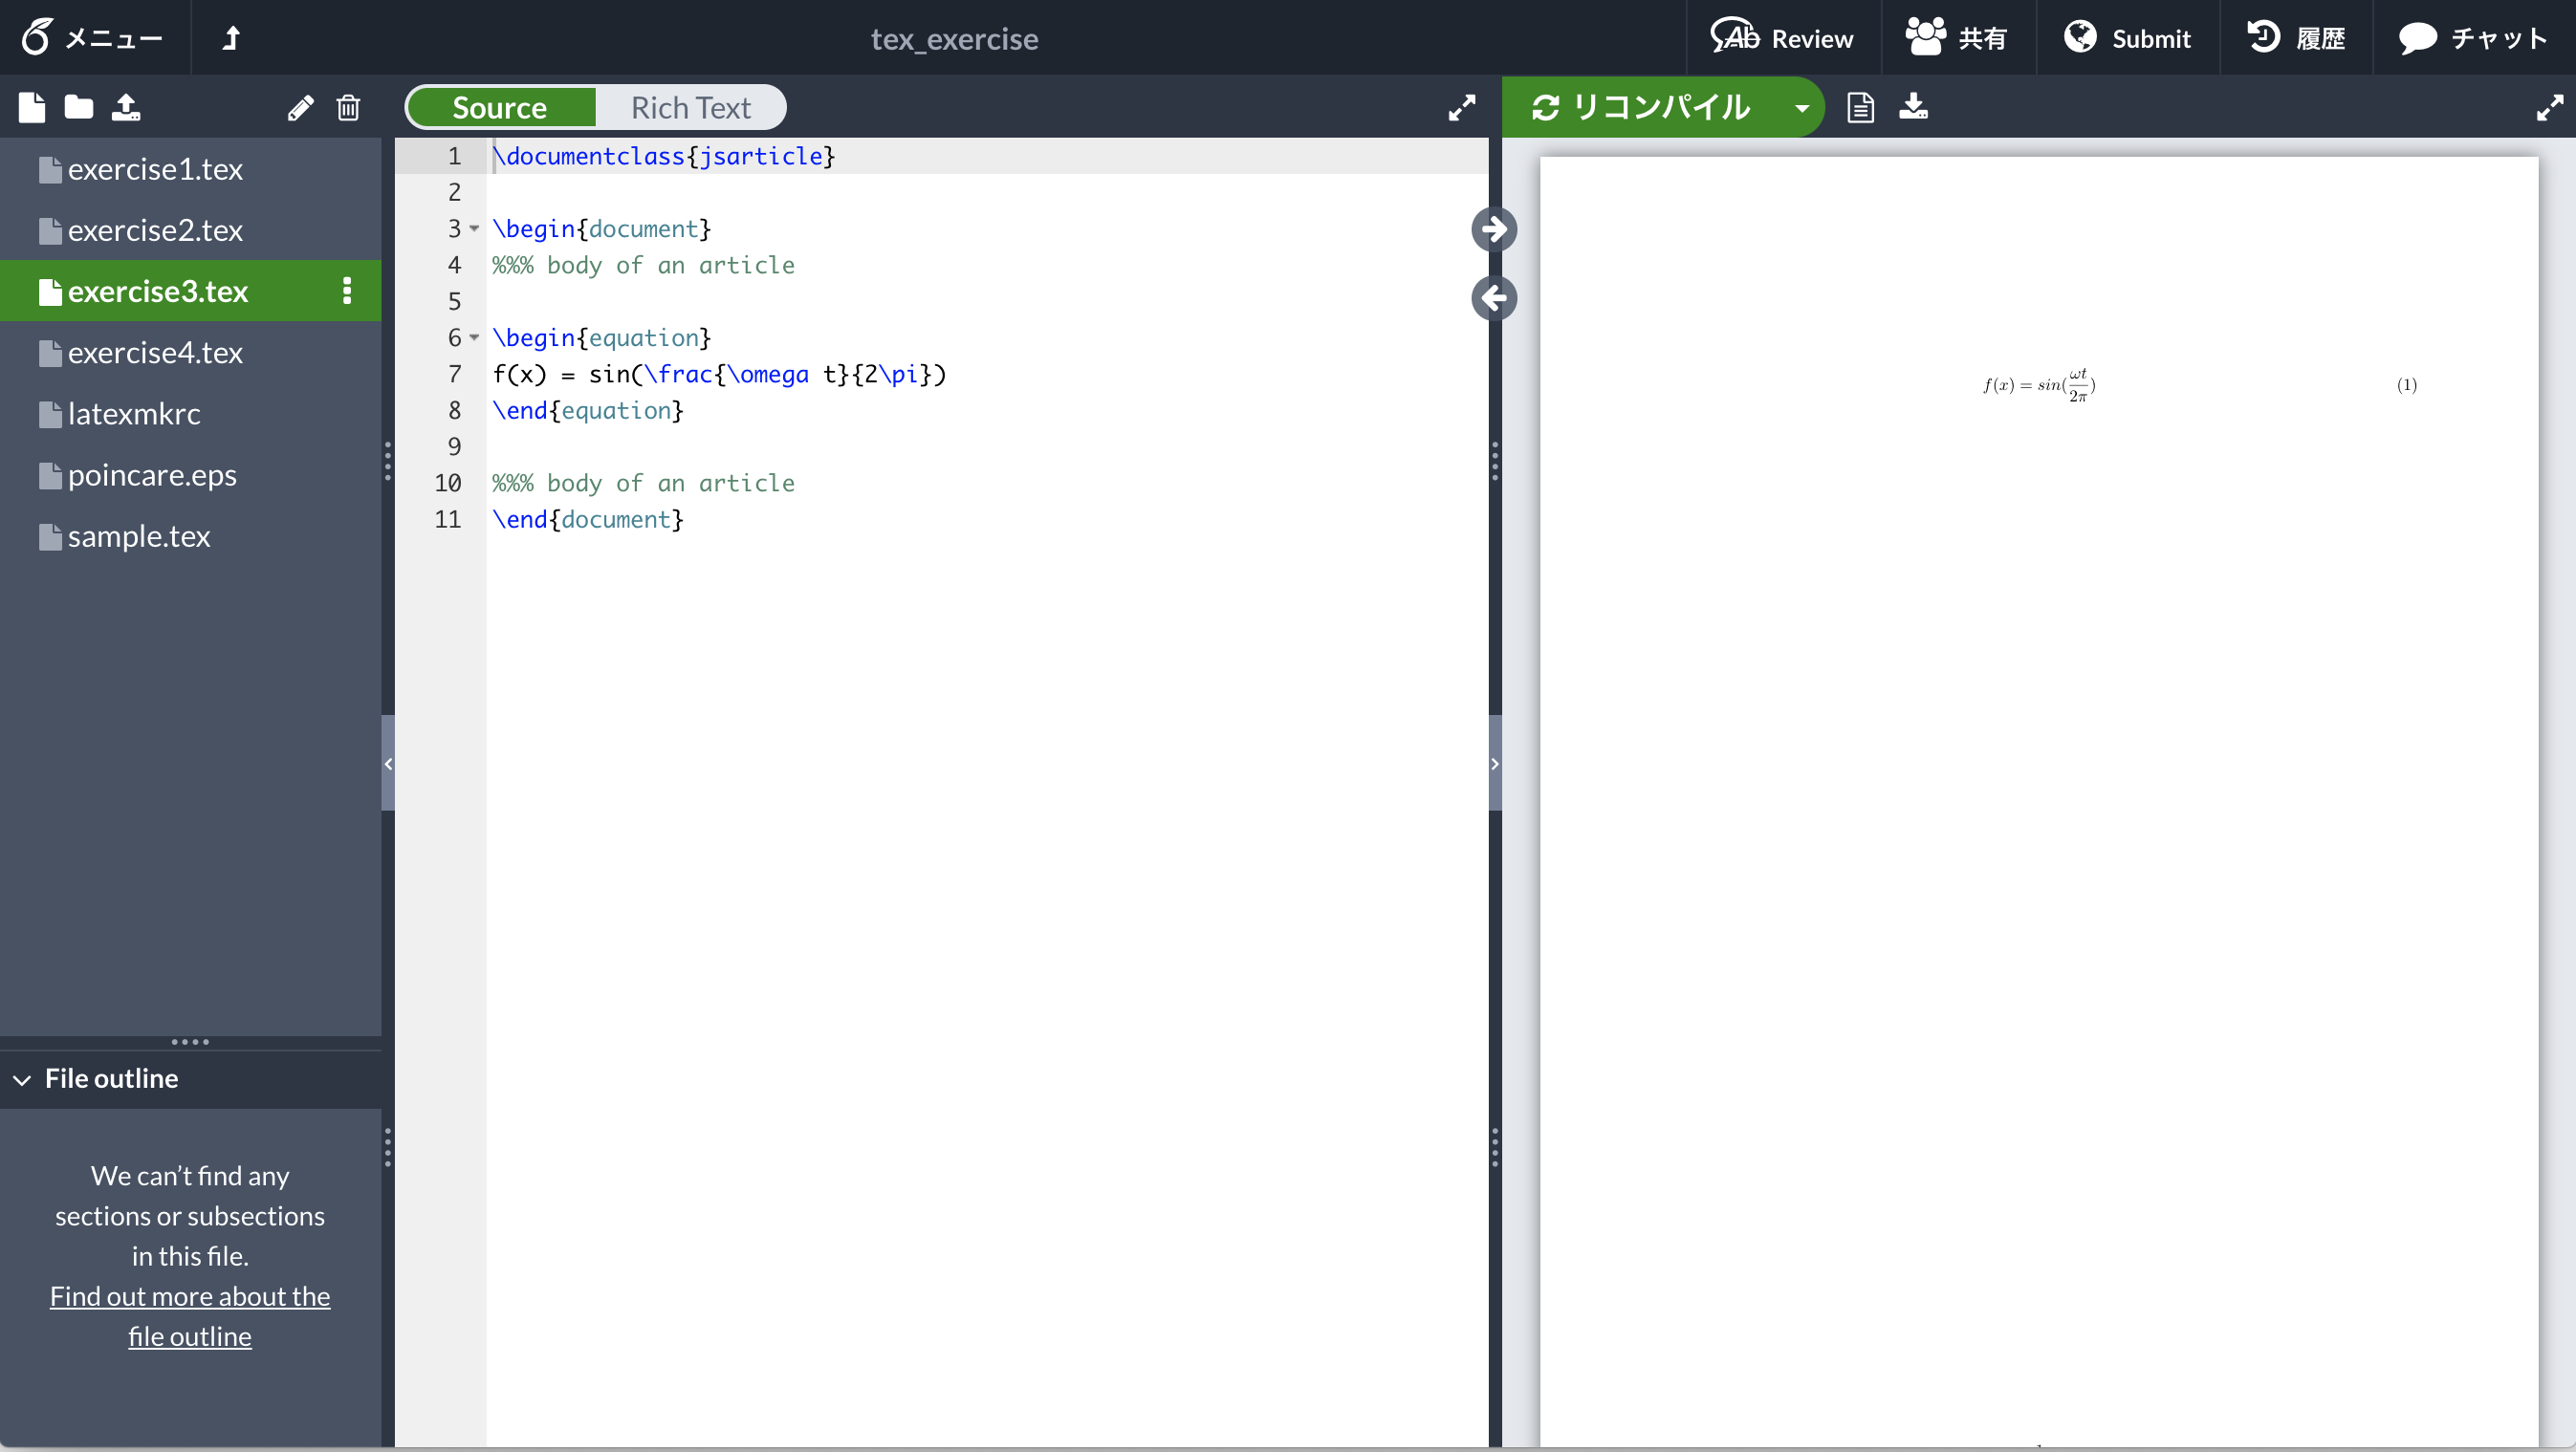
\includegraphics[width=100mm]{overleaf_start.png}
  \caption{\textbf{Overleaf}の作業画面}
  \label{overleaf}
\end{figure}
デフォルトでは日本語文章に対応していないため設定を変更しましょう。左上のメニューから\textbf{コンパイラ}で\textbf{LaTeX}を選択します。この設定と\underline{latexmkrc}という設定ファイルをプロジェクト内に置くことによって日本語文章を作成することができます。(今後別のプロジェクトで作業する際も同様の設定と、プロジェクト内にlatexmkrcを置いておくようにしましょう。)

\subsection{文章作成の流れ}
左上の\textbf{新規ファイル}からsample.texというファイルを作成し、左側のソースファイルの中身を次のようにします。
大文字・小文字も正確に入力してください。
\begin{screen}
\begin{verbatim}
\documentclass{jsarticle}
\begin{document}
こんにちは{\TeX}。はじめまして。
\end{document}
\end{verbatim}
\end{screen}

次に右枠上部の\textbf{リコンパイル}を押すことで、右側のプレビューに図\ref{hello}のように表示されます。これで文書の作成は完了です。

最後に右枠上部のダウンロードアイコンから作成したpdfファイルをダウンロードできます\footnote{メニューからソースファイルの一括ダウンロードもできます}。
このときファイル名はソースファイル名(sample)ではなくプロジェクト名(tex\_exercise)から取られます。
\begin{figure}
  \centering
  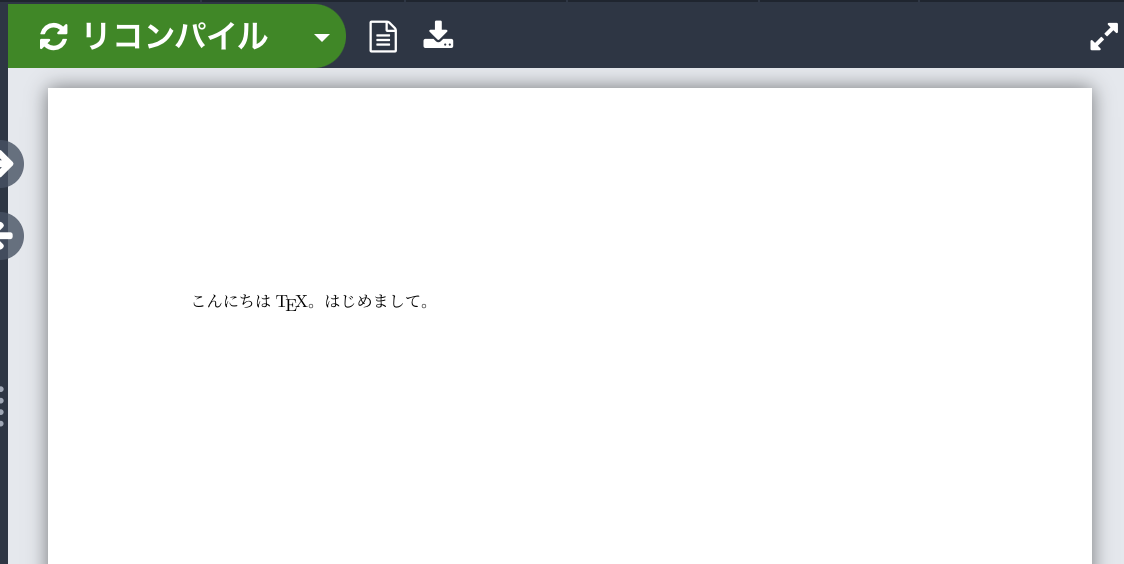
\includegraphics[width=100mm]{hellotex.png}
  \caption{pdfのプレビュー\label{hello}}
\end{figure}

\subsection{エラーに遭遇したら}
{\LaTeX}で文書を作成していると、しょっちゅうエラーに
遭遇します。このときの対処方法を覚えましょう。

先ほどのsample.texの2行目を少しだけ変えてみます。
\begin{screen}
\begin{verbatim}
\documentclass{jsarticle}
\began{document}
こんにちは{\TeX}。はじめまして。
\end{document}
\end{verbatim}
\end{screen}
これで\textbf{リコンパイル}を押すと図\ref{hello}とは異なる結果が表示されるでしょう。
このように思い通りに文章が作成されない時は再編集ボタンの右の\textbf{ログと出力ファイル}を見ます。
おそらく一つ目にこんなふうに言われていることでしょう。
\begin{screen}
\begin{verbatim}
Undefined control sequence. sample.tex, line 2

<recently read> \began

l.2 \began
          {document}
The control sequence at the end of the top line
of your error message was never \def'ed. If you have
misspelled it (e.g., `\hobx'), type `I' and the correct
spelling (e.g., `I\hbox'). Otherwise just continue,
and I'll forget about whatever was undefined.
\end{verbatim}
\end{screen}
こんなときは、表示された説明をよく読みます。今の場合は
\verb+begin+という
ところを\verb+began+と書いたため、怒られているようです。\verb+l.2+(2行目)
というのもヒントになりますね。さらに二つ目のログで
\begin{screen}
  \begin{verbatim}
LaTeX Error: Missing \begin{document}.
\end{verbatim}
\end{screen}
と言われているところからも原因を突き止めることができます。
こんな時はソースファイルに戻り、間違いを直してからもう一度\textbf{リコンパイル}を押します。
\pagebreak

%section 2
%%%%%%%%%%%%%%%%%%%%%%%%%%%%%%%%%%%%%%%%%%%%%%%%%%%%%%%%%%%%%%%%%%%%%%%%%%%%%%%%
%%%%%%%%%%%%%%%%%%%%%%%%%%%%%%%%%%%%%%%%%%%%%%%%%%%%%%%%%%%%%%%%%%%%%%%%%%%%%%%%

\section{はじめに}
1章にしたがって使えば、とりあえず動くようにはなります。
しかし、少しは{\LaTeX}の歴史を知っておくのもよいでしょう。

\subsection{{\TeX} とは}
{\TeX}\footnote{手書きなどで{\TeX}というロゴが出力できないときは、\emph{必ず} `TeX'のようにeだけを小文字にして書きます。同様に{\LaTeX}は`LaTeX'と書きます。まあ`KinKi Kids'みたいなもんです。}というソフトは、\verb+Stanford+大学の\verb+Donald E. Knuth+教授(当時)が作成した文書組版用ソフトウェアです。
{\TeX}をどう発音するかはなかなか難しい問題なのですが、これはギ
リシャ語の$\tau$と$\epsilon$と$\chi$をくっつけった発音になるのだそうです。
日本語にも英語にも$\chi$という音はないので、だいたい「てっく」とか「てふ」
と発音します。

組版(typesetting)というのはあまり聞き慣れない言葉ですが、もともと印刷用語で、
活字を組んで紙面を構成することを指します。{\TeX}はこれをコンピュータの上で行うための
ソフトウェアです。

{\TeX}には次のような特徴があります:
\begin{itemize}
 \item {\TeX}はフリーソフトなので、無料で入手できます。インストールの方法
       も日進月歩で進化しており、ご家庭のパソコンにも簡単にインストール
       できます\footnote{TeXLiveやMacTeXなどで調べてみてください。}。
 \item WindowsやMacintosh、UNIXなど様々なプラットフォームで、まったく同
       じ出力が得られます。
 \item 特に数式の美しさは変態的です。出版の専門家でない我々が
\begin{equation}
 \frac{d}{dt} \Phi (t) = \lim_{\delta t \rightarrow 0} \frac{\Phi(t +
  \delta t) - \Phi(t)}{\delta t} \\
    =  \int_{S(t)} \left( \frac{\partial}{\partial t} \vec{B} -
		      \vec{\nabla} \times (\vec{U} \times
		      \vec{B})  \right) \cdot
    d \vec{S} = 0 \nonumber
\end{equation}
       とか書けてしまうのはすばらしいことです。
 \item `dif{}ferent'や`f{}inish'が、それぞれ`different'や`finish'となる
       ように、`ff'や`fi'は文字がくっついたデザインになります。これを
       \emph{リガチャ}(合字)といます。{\TeX}は
       これを自動で行います。
 \item \emph{カーニング}(字詰め)も自動で行い、`V{}olcano'は`Volcano'の
       ようにoがVの下に入ります。
 \item 最適な改行・最適な改ページをしてくれます。たとえば、段落の最後の1行だけが
       次のページになってしまう、というようなことは避けられます。
\end{itemize}
このようにレイアウトに関しては{\TeX}がやってくれるので、我々は文書の中身を作ることに
専念できるのです。その代わりにこのような計算にはそれなりに手間がかかりますから、
「1文字打ったら則画面に反映される」ような方法では、計算機には多大な負荷
がかかるでしょうし、我々は眼が疲れるでしょう。
そこで「ある程度できた段階でまとめて{\TeX}に処理してもらう」という方法
をとっています。

\subsection{\LaTeX とは}

裸の{\TeX}は非常に完成度の高いプログラミング言語です。完成度が高いという
ことは裏を返せば一つのことを実現するのにたいへん多くの手順が必要である
ということです。これでは実用上やや問題がありますので、基本的(primitive)な{\TeX}の
機能を組み合わせてあらかじめ機能強化をしておいたほうが実用的です。

DEC(Digital Equipment Corporation)のコンピュータ科学者
Leslie Lamportは文書作成が簡単に行え
るように{\TeX}を機能強化し、{\LaTeX}というシステムを開発しました。
{\LaTeX}の発音は{\TeX}に倣って、「らてっく」とか「らてふ」でよいと思いま
す。
{\LaTeX}は、ウェブ上で使われているHTML(HyperText Markup Languege)と同じ
ようにマークアップ言語です。したがって雰囲気は似ていて、HTMLだと
\begin{screen}
\begin{verbatim}
<CENTER>中央揃え</CENTER>
\end{verbatim}
\end{screen}
となるのが、{\LaTeX}では
\begin{screen}
\begin{verbatim}
\begin{center}中央揃え\end{center}
\end{verbatim}
\end{screen}
のようになるわけです。

{\LaTeX}の初期バージョンは2.09で、現在も書籍部で{\LaTeX}の古典的な本を見
てみれば{\LaTeX}2.09の記述を発見できると思います。その後1993年には
{\LaTeXe}というバージョンにバージョンアップしました。本書ではこのシステ
ムを説明します。

\subsection{\TeX と日本語}
(株)アスキーによって日本語化された{\TeX}の仲間は、頭にp(ピー,publishing
の意)がつきます。設定ファイルlatexmkrcにあるplatexというのは、{\LaTeX} を日本
語用に修正したものなわけです。

\pagebreak

%section 3
%%%%%%%%%%%%%%%%%%%%%%%%%%%%%%%%%%%%%%%%%%%%%%%%%%%%%%%%%%%%%%%%%%%%%%%%%%%%%%%%
%%%%%%%%%%%%%%%%%%%%%%%%%%%%%%%%%%%%%%%%%%%%%%%%%%%%%%%%%%%%%%%%%%%%%%%%%%%%%%%%

\section{\LaTeX の基本(1)}

\subsection{文書の構造}
1.2節において、{\LaTeX}の文書は以下のように作るという説明
をしました。
\begin{screen}
\begin{verbatim}
\documentclass{jsarticle}
\begin{document}

\end{document}
\end{verbatim}
\end{screen}
もう少し正確にいうと、{\LaTeX}の文書は以下のような構造をしています。
\begin{screen}
\begin{verbatim}
\documentclass[オプション]{クラス}
「プリアンブル」
\begin{document}
「本体」
\end{document}
\end{verbatim}
\end{screen}
まずはこの説明からしましょう。

\subsection{ドキュメントクラス}
\verb+\documentclass+の部分では、どのような用途の文書を作成したいかを指
定します。例えばちょっとしたレポートなら、上下左右にてきとうに空白が開い
てページ下の中央にページ番号が入ればよいですが、本を作成するとなれば右ペ
ージと左ページで余白の大きさは違うでしょうし、ページ番号も外側に出力し
たくなるでしょう。

このように、文書の大まかな書式を\emph{クラス}といいます.\verb+{クラス}+の
部分には、以下のようなものが指定できます。\\
\begin{description}
 \item[jsarticle] 和文のレポート・雑誌記事など、当面ほとんどの用途はこれ
 \item[jsbook] 和文の書籍や論文;論文は後述のオプションにreportを指定する
 \item[article] 欧文のレポート、雑誌記事など
 \item[report] 欧文の論文など
 \item[book] 欧文の書籍;ページ数の偶奇で余白が異なる
\end{description}
\verb|article|、\verb|report|、\verb|book|は欧文用で、
余白のとり方、段落の下がり方などがちょっと違います。和文用クラスには、\verb|jarticle|、\verb|jreport|、\verb|jbook|というものもありますが、より新しく改良されている\verb|jsarticle|、\verb|jsbook|を用いた方が良いようです。

また、大まかに書式は同じでも文字の大きさだけ変えたいとか、用紙サイズだけ
変えたい、などという希望もあると思います。これは\verb+[オプション]+の部分で指定
します。\verb+[オプション]+にはいろいろなものが指定できますが、少しだけ紹介
すると、
\begin{description}
 \item[文字サイズ] 10pt, 11pt, 12ptのいずれか
	    が使えます。何も指定しなければ10ptです。
 \item[用紙サイズ]  a4paper, b5paper, a5paper,
	    letterpaperなどが使えます。何も指定しなければ
	    a4paperです。
\item[段組] onecolumnなら1段組、twocolumnなら2段組です。
	    何も指定しなければonecolumnです。
\item[用紙方向] landscapeなら横長の向きになります。何も指定しな
	    ければ縦長です。
\end{description}
のようになります。\verb+[オプション]+は``,''で区切って複数の
\verb+[オプション]+を指定することが可能です。

\subsection{タイトル}
文書を作るときは、\emph{表題}、\emph{作者}、\emph{日付}を書くのが一般的
です。プリアンブルの部分に
\begin{screen}
\begin{verbatim}
\title{表題}
\author{作者}
\date{日付}
\end{verbatim}
\end{screen}
を記述しておいてから、\verb+\begin{document}+のあとで
\begin{screen}
\begin{verbatim}
\maketitle
\end{verbatim}
\end{screen}
とすることで書くことができます。

\subsection{見出し}

ちょっとしたメモはともかくとして、ある程度まとまった文章を書こうとした場
合、まず「章」があって、その次に「節」があって…、というように論理的に組
み立てていくことが大切になります。
{\LaTeX}ではこの作業を半自動的に行うコマンドが用意されています。
表\ref{tab:headline}に示すような命令を使うと,見出し用に文字の大きさな
どがわかり、番号も自動的に振られます。
\begin{table}[htbp]
\begin{center}
\caption{{\LaTeX}での見出しの定義の種類}
\label{tab:headline}
\begin{tabular}{c|c}\hline
 \verb+\part{見出し}+         & 部 \\
 \verb+\chapter{見出し}+       & 章${}^{*}$ \\
 \verb+\section{見出し}+       & 節 \\
 \verb+\subsection{見出し}+    & 小節 \\
 \verb+\subsubsection{見出し}+ & 小小節 \\
 \verb+\paragraph{見出し}+     & 段落 \\
 \verb+\subparagraph{見出し}+  & 小段落 \\
 \hline
\end{tabular}\\
{\small ${}^{*}$\verb+(js)article+には章は定義されていません}
\end{center}
\end{table}

使用例を見てみましょう。\\
\begin{minipage}[c]{.50\textwidth}
\begin{screen}
\small
\begin{verbatim}
\section{はじめに}
 ハナ肇の話をしましょう。
 \subsection{経歴}
 \subsection{クレイジーキャッツ}
\section{おわりに}
 \subsection{最近の旅行}
 尾張に行きました。
\end{verbatim}
\end{screen}
\end{minipage}
%\manerarrow\hfill{}
$\Rightarrow$
\begin{minipage}{.45\textwidth}
\begin{shadebox}
{\Large \textbf{1 はじめに}}\\
ハナ肇の話をしましょう.\\
\hspace*{1em}{\large \textbf{1.1 経歴}}\\
\hspace*{1em}{\large \textbf{1.2 クレイジーキャッツ}}\\
\vspace*{-0.4zw}\\
{\Large \textbf{2 おわりに}}\\
\hspace*{1em}{\large \textbf{2.1 最近の旅行}}\\
\hspace*{1em}{尾張に行きました.}
\end{shadebox}
\end{minipage}
\vspace*{1mm}\\
番号が振られ、文字が太字になり、見出しの階層に応じてサイズが大きくなりました。さら
に、あとから一つ節を加えると、\\
\begin{minipage}[c]{.50\textwidth}
\begin{screen}
\small
\begin{verbatim}
\section{はじめに}
 ハナ肇の話をしましょう.
 \subsection{経歴}
 \subsection{クレイジーキャッツ}
\section{なかに}
\section{おわりに}
 \subsection{最近の旅行}
 尾張に行きました.
\end{verbatim}
\end{screen}
\end{minipage}%
%\manerrarrow\hfill{}
$\Rightarrow$
\begin{minipage}{.45\textwidth}
\begin{shadebox}
{\Large \textbf{1 はじめに}}\\
ハナ肇の話をしましょう.\\
\hspace*{1em}{\large \textbf{1.1 経歴}}\\
\hspace*{1em}{\large \textbf{1.2 クレイジーキャッツ}}\\
\vspace*{-0.4zw}\\
{\Large \textbf{2 なかに}}\\
\vspace*{-0.4zw}\\
{\Large \textbf{3 おわりに}}\\
\hspace*{1em}{\large \textbf{3.1 最近の旅行}}\\
\hspace*{1em}{尾張に行きました.}
\end{shadebox}
\end{minipage}
\vspace*{1mm}\\
というように番号が変わります。したがって{\LaTeX}では番号の振り間違いはあ
りえません。このおかげで、\emph{内容の編集に集中できる}のです\footnote{\verb+\section*{}+というように\verb+*+を挟むことで番号を振らないようにすることもできます。}。

\subsection{改行の扱い}
ワープロソフトでは\keytop{Enter}を押せば行が変わって表示
されますし、印刷すれば実際にそこで改行されていることがわかります。
しかし{\TeX}は前述の通り、どこで改行すべきかをある規則にのっとって自動的
に計算します。例えば、単語の途中で改行してはいけないですし、ある行は40文
字なのに次の行は20文字しかない、というのもキモイです。
したがって基本的に、\emph{自分で入力した改行は無視されます}。通常は入力
画面の右端に近づいたら改行すればよいですし、電子メールのように区切りのよ
いところで改行するのもよいでしょう。
ただし、改行だけの(\keytop{Enter}だけが入力してある)行があると、{\TeX}
はこれを段落の区切りと解釈します。

では具体例を見てみましょう: \\

\begin{minipage}[c]{.50\textwidth}
\begin{screen}
\small
\begin{verbatim}
改行は
無視されます。
どんなに
ぶち
ぶち
切っても
へっちゃらで
す。
ただし何も入力しない行があると

段落の区切りと解釈し、次の段落が始まります。
\end{verbatim}
\end{screen}
\end{minipage}%
%\manerrarrow\hfill{}
$\Rightarrow$
\begin{minipage}{.45\textwidth}
\begin{shadebox}
改行は
無視されます。
どんなに
ぶち
ぶち
切っても、
へっちゃらで
す。
ただし何も入力しない行があると

段落の区切りと解釈し、次の段落が始まります。
\end{shadebox}
\end{minipage}
\vspace*{1mm}\\

もしどうしても強制的に改行したい場合は、\verb+\\+とバックスラッシュを2個
続けて入力すればいいのですが、これは慎重にやったほうがよいでしょう。

\subsection{空白の扱い}
空白はやや丁寧に考えてみましょう。いま、英文を入力しようと思ったとします
。ワープロソフトを用いた場合、単語の間には通常半角空白を1つ入れるでしょ
う。また、センテンスとセンテンスの間には単語間よりも大きめの空白を入れま
すから、タイプライタではふつう、半角空白を2つ入れます。{\LaTeX}では単語
の区切りさえ示しておけば、これらの作業が半自動で行われます。例えば1998年
度の東京大学入試問題の一節をタイプセットしてみると、次のようになります
%(\verb*+ +は空白が入力されていることを示します)
。\\
\begin{minipage}[c]{.50\textwidth}
\begin{screen}
\small
\begin{verbatim}
Simple Peter held the mirror up to
his face and peered into it. First he
turned one way, then he turned the
\end{verbatim}
\end{screen}
\end{minipage}%
%\manerrarrow\hfill{}
$\Rightarrow$
\begin{minipage}{.45\textwidth}
\begin{shadebox}
Simple Peter held the mirror up to
his face and peered into it. First he
turned one way, then he turned the
\end{shadebox}
\end{minipage}
\vspace*{1mm}\\
上の文章はすべて空白を1つずつしか入れていませんが、{\LaTeX}は``it''と
``First''の間を大きくしていることがわかると思います。また、1行目と2行目
とで右端もきちんとそろっています。
ですから結論から言うと、\emph{空白は}{\LaTeX}\emph{に任せる}べきです。

そうはいっても、どうしても空白を作りたいこともあると思います。そんなとき
は、空白を\verb|\|で区切ります。例えば\verb|\|を5個書けば、
半角空白が6個分出力されます。また、空白の途中で改行されては困るときは、
\verb|~|を入力します。\verb|~|であけた空白では改行が起こりません。
具体的にはこんな感じです。\\

\begin{minipage}[c]{.50\textwidth}
\begin{screen}
\small
\begin{verbatim}
Fill in the blank below:\\
So Peter (                      ).\\
これでは残念賞。\\
So Peter ( \ \ \ \ \ \ \ \ \ \ \ ).\\
So Peter (~~~~~~~~~~~~).\\
これなら書き込めるぞ。
\end{verbatim}
\end{screen}
\end{minipage}%
%\manerrarrow\hfill{}
$\Rightarrow$
\begin{minipage}{.45\textwidth}
\begin{shadebox}
Fill in the blank below:\\
So Peter (                      ).\\
これでは残念賞。\\
So Peter ( \ \ \ \ \ \ \ \ \ \ \ ).\\
So Peter (~~~~~~~~~~~~).\\
これなら書き込めるぞ。
\end{shadebox}
\end{minipage}
\vspace*{1mm}\\

\subsection{練習}
ここまでの練習をしましょう。プロジェクトtex\_exerciseの中にある\underline{exercise1.tex}を適当に編集してみてください。具体的には
\begin{itemize}
 \item[-] \verb+\title+などを自分仕様に変えてみる
 \item[-] \verb+\date+を省略するとどんな振る舞いをするか観察する
 \item[-] \verb+\section+やら\verb+\subsection+やらを使ってみる
 \item[-] 改行や空白を適宜放り込んで振る舞いを観察する
\end{itemize}
などという作業をやってみてください。

\pagebreak

%section 4
%%%%%%%%%%%%%%%%%%%%%%%%%%%%%%%%%%%%%%%
%%%%%%%%%%%%%%%%%%%%%%%%%%%%%%%%%%%%%%%

\section{\LaTeX の基本(2)}

\subsection{特別な意味を持つ記号}
ここまでの話で\verb+\+とか\verb+{+とか\verb+}+といった記号には特別な意
味があって、その記号自体は出力されないということに気づいた人もいるかも
しれません。それは正解で、
\begin{quote}
\verb+\ { } $ & # ^ _ ~ %+
\end{quote}
の10文字はそのまま入力することはできません。このうち、\verb+\+、\verb+^+、
\verb+~+以外は文字の前に\verb+\+をつけることで対処できます。

\subsection{特殊記号の入力}
もう少し勘のよい人は、{\LaTeX}というロゴはどうやって出力しているのだろう
と疑問に思うかもしれません。{\LaTeX}には表\ref{tab:char}に示すように、
いくつかの特殊記号・特殊文字が定義されています。
\begin{table}[htbp]
\begin{center}
\caption{{\LaTeX}で利用できる特殊記号}
\label{tab:char}
\begin{tabular}{ll|ll|ll|ll|ll}%\hline
\verb+\{+ & \{ & \verb+\aa+ & \aa & \verb+\l+  & \l  & \verb+\dag+  & \dag  & \verb+!`+         & !`         \\
\verb+\}+ & \} & \verb+\AA+ & \AA & \verb+\L+  & \L  & \verb+\ddag+ & \ddag & \verb+?`+         & ?`         \\
\verb+\$+ & \$ & \verb+\ae+ & \ae & \verb+\o+  & \o  & \verb+\S+    & \S    & \verb+\pounds+    & \pounds    \\
\verb+\&+ & \& & \verb+\AE+ & \AE & \verb+\O+  & \O  & \verb+\P+    & \P    & \verb+\copyright+ & \copyright \\
\verb+\#+ & \# & \verb+\oe+ & \oe & \verb+\ss+ & \ss & \verb+\i+    & \i    & \verb+\TeX+       & \TeX       \\
\verb+\_+ & \_ & \verb+\OE+ & \OE & \verb+\SS+ & \SS & \verb+\j+    & \j    & \verb+\LaTeX+     & \LaTeX     \\
\verb+\%+ & \% &            &     &            &     &              &       & \verb+\LaTeXe+    & \LaTeXe
\end{tabular}
\end{center}
\end{table}

\subsection{書体}
{\LaTeX}では書体の種類は、
\begin{description}
\item[ファミリー] 文字のデザインの違い;``{\rmfamily NHK}''にはひげがあ
	   るけど``{\sffamily NHK}''にはひげがない
\item[シリーズ] 文字の太さの違い;``{\bfseries YKK}''は太くて
	   ``{\mdseries YKK}''は細い
\item[シェイプ] 形状の違い;``{\itshape This}''はイタリックで``{\scshape 
	   This}''は小文字も大文字と同じ形
\end{description}
の3種類に分けられます。書体を変更したいときは
\begin{screen}
\begin{verbatim}
\書体を変更する命令{変更したい文字列}
\end{verbatim}
\end{screen}
のように書きます。\emph{書体を変更する命令}は表\ref{tab:design}に示すようなものがあります。

これらの命令を使って、次のように書体を変更できます。\\
\begin{minipage}[c]{.50\textwidth}
\begin{screen}
\small
\begin{verbatim}
She is my mother, but I am
\textbf{not} her daughter.\\
She is my mother, but I am
\textit{not} her daughter.
\end{verbatim}
\end{screen}
\end{minipage}%
%\manerrarrow\hfill{}
$\Rightarrow$
\begin{minipage}{.45\textwidth}
\begin{shadebox}
She is my mother, but I am
\textbf{not} her daughter.\\
She is my mother, but I am
\textit{not} her daughter.
\end{shadebox}
\end{minipage}
\vspace*{1mm}\\
また、これらの命令は組み合わせて使うこともでき、例えば「太字でイタリック
にしたい」と思ったときは次のようにします。\\
\begin{minipage}[c]{.50\textwidth}
\begin{screen}
\small
\begin{verbatim}
She is my brother, but I am
\textbf{\textit{not}} her daughter.
\end{verbatim}
\end{screen}
\end{minipage}%
%\manerrarrow\hfill{}
$\Rightarrow$
\begin{minipage}{.45\textwidth}
\begin{shadebox}
She is my mother, but I am
\textbf{\textit{not}} her daughter.
\end{shadebox}
\end{minipage}
\vspace*{1mm}\\
\begin{table}[htbp]
\begin{center}
\caption{書体の変更}
\label{tab:design}
\begin{tabular}{lll}
\hline
書体名                     & 命令         & 出力例                       \\
\hline
ローマンファミリー         & \verb+\textrm+ & \textrm{This is Roman.}      \\
サンセリフファミリー       & \verb+\textsf+ & \textsf{This is San Serif.}  \\
タイプライタファミリー     & \verb+\texttt+ & \texttt{This is Typewriter.} \\
\hline
ミディアムシリーズ         & \verb+\textmd+ & \textmd{This is Mediumface.} \\
ボールドシリーズ           & \verb+\textbf+ & \textbf{This is Boldface.}   \\
\hline
イタリックシェイプ         & \verb+\textit+ & \textit{This is Italic.}     \\
スラントシェイプ           & \verb+\textsl+ & \textsl{This is Slanted.}    \\
スモールキャピタルシェイプ & \verb+\textsc+ & \textsc{This is Small Caps.} \\
\hline
\end{tabular}
\end{center}
\end{table}

一方、全角文字は標準では明朝とゴシックしかなく、表\ref{tab:design2}の命
令を使います。以下に使用例を示します。\verb+\textmc+はなにもしないのと同じです。\\
\begin{table}[htbp]
\begin{center}
\caption{全角文字の書体の変更}
\label{tab:design2}
\begin{tabular}{lll}
\hline
書体名             & 命令         & 出力例                    \\
\hline
明朝ファミリー     & \verb+\textmc+ & \textmc{明朝体です。}     \\
ゴシックファミリー & \verb+\textgt+ & \textgt{ゴシック体です。} \\
\hline
\end{tabular}
\end{center}
\end{table}
\\
\begin{minipage}[c]{.50\textwidth}
\begin{screen}
\small
\begin{verbatim}
強調したいところは\textgt{ゴシック体}を
使います。
\end{verbatim}
\end{screen}
\end{minipage}%
%\manerrarrow\hfill{}
$\Rightarrow$
\begin{minipage}{.45\textwidth}
\begin{shadebox}
強調したいところは\textgt{ゴシック体}を
使います。
\end{shadebox}
\end{minipage}
\vspace*{1mm}\\

\subsection{文字の大きさ}
もちろん文字の大きさも変更できます。文字の大きさを変更するには、
\begin{screen}
\verb+{\+文字の大きさを変える命令 (変えたい文字)\verb+}+
\end{screen}
のようにします。\emph{文字の大きさを変える命令}は表\ref{tab:size}に示
すように10種類あります。\verb+\normalsize+は何もしないのと同じです。\\
\begin{table}[htbp]
\begin{center}
\caption{文字の大きさの変更}
\label{tab:size}
\begin{tabular}{lll}
\hline
 命令 & 出力例 & 使うべき要素(参考) \\
\hline
 \verb+\tiny+         & {\tiny とても小さい}       & 振り仮名           \\
 \verb+\scriptsize+   & {\scriptsize かなり小さい} &                    \\
 \verb+\footnotesize+ & {\footnotesize 小さい}     & 脚注               \\
 \verb+\small+        & {\small 少し小さい}        & 図表見出し         \\
 \verb+\normalsize+   & {\normalsize 普通}         & 本文・小小節見出し \\
 \verb+\large+        & {\large 少し大きい}        & 小節見出し         \\
 \verb+\Large+        & {\Large 大きい}            & 節見出し           \\
 \verb+\LARGE+        & {\LARGE とても大きい}      &                    \\
 \verb+\huge+         & {\huge かなり大きい}       &                    \\
 \verb+\Huge+         & {\Huge 超大きい}           & 章・節見出し       \\
\hline
\end{tabular}
\end{center}
\end{table}
ただし、無意味に文字の大きさを変えても読みにくくなるだけです。文字の大き
さを変えると、例えば次のようなことができます。\\
\begin{minipage}[c]{.50\textwidth}
\begin{screen}
\small
\begin{verbatim}
テーブルから紙ナプキンが
{\tiny ど}
{\scriptsize ん}
{\footnotesize が}
{\small ら}
{\normalsize が}
{\large っ}
{\Large し}
{\LARGE ゃ}
{\huge ー}
{\Huge ん}
と落ちた。
\end{verbatim}
\end{screen}
\end{minipage}%
%\manerrarrow\hfill{}
$\Rightarrow$
\begin{minipage}{.45\textwidth}
\begin{shadebox}
テーブルから紙ナプキンが
{\tiny ど}
{\scriptsize ん}
{\footnotesize が}
{\small ら}
{\normalsize が}
{\large っ}
{\Large し}
{\LARGE ゃ}
{\huge ー}
{\Huge ん}
と落ちた。
\end{shadebox}
\end{minipage}
\vspace*{1mm}\\
表\ref{tab:size}には、標準の設定にしたときに文書中のどの要素でどの大き
さが使われるかも書いておきましたので、参考にしてください。

\subsection{脚注}
脚注をつけるには、つけたいところに
\begin{screen}
\begin{verbatim}
脚注をつけたい文字列\footnote{脚注の内容}
\end{verbatim}
\end{screen}
のように書きます\footnote{こんなふうに書きます。}。番号は自動的に振ら
れます。

\subsection{コメント}
もとのファイルに何かコメントを残しておきたい場合、\verb+%+につづけて書き
ます。この部分は何を書いても出力されません。次の例が理解できれば大丈夫でしょう。\\
\begin{minipage}[c]{.50\textwidth}
\begin{screen}
\small
\begin{verbatim}
ここは出力されますが%ここは出力されない。
%この行は丸ごとコメントなので
出力されないでしょう。
\end{verbatim}
\end{screen}
\end{minipage}%
%\manerrarrow\hfill{}
$\Rightarrow$
\begin{minipage}{.45\textwidth}
\begin{shadebox}
ここは出力されますが%ここは出力されない。
%この行は丸ごとコメントなので
出力されないでしょう。
\end{shadebox}
\end{minipage}
\vspace*{1mm}\\

\subsection{引用}
一般的に単語を引用したい場合、シングルクオート` 'を使いますし、一文を引
用したいときはダブルクオート`` ''を使います。ところが、キーボードを見て
みるとわかりますが、`という記号はどこにもありません。ためしに
\keytop{Shift}$+$\keytop{7}の\keytop{'}と\keytop{Shift}$+$\keytop{2}の
\keytop{"}とで何とかしてみようと思うと、\\
\begin{minipage}[c]{.50\textwidth}
\begin{screen}
\small
\begin{verbatim}
Bob said, "This 'B' is strange".
\end{verbatim}
\end{screen}
\end{minipage}%
%\manerrarrow\hfill{}
$\Rightarrow$
\begin{minipage}{.45\textwidth}
\begin{shadebox}
Bob said, "This 'B' is strange".
\end{shadebox}
\end{minipage}
\vspace*{1mm}\\
のように引用の始まりも終わりも同じになってがっかりしてしまいます。

正しくは、引用の始まりには\keytop{Shift}$+$\keytop{@}の\emph{バッククオ
ート}\keytop{`}を使います。終わりはそのまま\keytop{Shift}$+$\keytop{7}の
\keytop{'}でかまいません。
この2文字の組をシングルクオートの場合は1つずつ、\emph{ダブルクオートの場
合は2つずつ}入力します。\emph{決して}\keytop{Shift}$+$\keytop{2}\emph{の}
\keytop{"}\emph{で代用してはいけません.}\\

\begin{minipage}[c]{.50\textwidth}
\begin{screen}
\small
\begin{verbatim}
Bob said, ``This `B' is strange''.
\end{verbatim}
\end{screen}
\end{minipage}%
%\manerrarrow\hfill{}
$\Rightarrow$
\begin{minipage}{.45\textwidth}
\begin{shadebox}
Bob said, ``This `B' is strange''.
\end{shadebox}
\end{minipage}
\vspace*{1mm}\\

\subsection{練習}
さっきのexercise1.texの書体、文字の大きさなどを適当に変えて遊んで
みましょう。

\pagebreak


%section 5
%%%%%%%%%%%%%%%%%%%%%%%%%%%%%%%%%%%%%%%
%%%%%%%%%%%%%%%%%%%%%%%%%%%%%%%%%%%%%%%

\section{環境}
これまで見てきたコマンドたちはみな、
\begin{screen}
\begin{verbatim}
\命令
\命令{引数}
\end{verbatim}
\end{screen}
という形をしていました。例えば、\verb+\maketitle+と書けば表題が表示されま
したし、\verb+\textbf{もじもじくん}+と書けば\textbf{もじもじくん}のよう
にゴシックになったわけです。これに対して、
\begin{itemize}
 \item[-] ある領域を全部中央揃えにしたい
 \item[-] ある領域を全部引用用に段落を下げたい
\end{itemize}
ということもあります。こんなときは、
\begin{screen}
\begin{verbatim}
\begin{環境}
  ある領域
\end{環境}
\end{verbatim}
\end{screen}
という\emph{環境型のコマンド}を使います。いくつか具体例を見ていきましょう。

\subsection{左揃え・中央揃え・右揃え}
とりあえず何かお知らせみたいなものを作成したいとき、この3つはよく使うと
思います。それぞれ表\ref{tab:flush}のような環境が用意されています。
\begin{table}[htbp]
\begin{center}
\caption{行を揃える環境}
\label{tab:flush}
\begin{tabular}{ll}
\hline
種類     & 環境             \\
\hline
左揃え   & \verb+flushleft+  \\
中央揃え & \verb+center+     \\
右揃え   & \verb+flushright+ \\
\hline
\end{tabular}
\end{center}
\end{table}

これらを使って、\\
\begin{minipage}[c]{.50\textwidth}
\begin{screen}
 \small
\begin{verbatim}
\begin{flushleft}
佐藤様 \\
鈴木様
\end{flushleft}

\begin{flushright}
2022年4月1日\\
地物太郎
\end{flushright}

\begin{center}
本年度の夏期賞与について
\end{center}
\end{verbatim}
\end{screen}
\end{minipage}%
%\manerrarrow\hfill{}
$\Rightarrow$
\begin{minipage}{.45\textwidth}
\begin{shadebox}
\begin{flushleft}
佐藤様 \\
鈴木様
\end{flushleft}

\begin{flushright}
2022年4月1日\\
地物太郎
\end{flushright}

\begin{center}
本年度の夏期賞与について
\end{center}

\end{shadebox}
\end{minipage}
\vspace*{1mm}\\
などと書くことができます。

\subsection{箇条書き}
長い長い文書の中に箇条書きを放り込むと、メリハリをつけることができます。
{\LaTeX}には
\begin{description}
 \item[itemize環境] 項目の頭に$\bullet$のようなマークをつける
	    \emph{記号つき箇条書き}です。入れ子にすると、それに伴って付
	    くマークも変わっていきます。
 \item[enumerate環境] 項目の頭に$1,2,3,\cdots$のような通し番号がつ
	    く\emph{番号つき箇条書き}です。入れ子にすると、それに伴って番
	    号がアルファベットになったりローマ数字になったりします。
 \item[description環境] 項目の頭が単語になっている\emph{説明つき箇
	    条書き}です。今のこの箇条書きが、まさにdescription環境
	    です。
\end{description}
という3つの箇条書き環境が用意されています。
これらはみな、
\begin{screen}
\begin{verbatim}
\begin{箇条書き環境名}
  \item[オプション]
\end{箇条書き環境名}
\end{verbatim}
\end{screen}
のように使います。

例えば、itemize環境を使うと、\\
\begin{minipage}[c]{.50\textwidth}
\begin{screen}
\small
\begin{verbatim}
我々の太陽系に属する天体は
\begin{itemize}
 \item planet
 \item dwarf planet
  \begin{itemize}
   \item ex) 冥王星,エリス
  \end{itemize}
 \item small solar system bodies
  \begin{itemize}
   \item 小惑星
    \begin{itemize}
     \item ex) リュウグウ
    \end{itemize}
   \item 彗星
   \item ほとんどのTNO
   \item その他の小天体
  \end{itemize}
\end{itemize}
に分類される(IAU Resolution 5A)
\end{verbatim}
\end{screen}
\end{minipage}%
%\manerrarrow\hfill{}
$\Rightarrow$
\begin{minipage}{.45\textwidth}
\begin{shadebox}
我々の太陽系に属する天体は
\begin{itemize}
 \item planet
 \item dwarf planet
  \begin{itemize}
   \item ex) 冥王星,エリス
  \end{itemize}
 \item small solar system bodies
  \begin{itemize}
   \item 小惑星
    \begin{itemize}
     \item ex) リュウグウ
    \end{itemize}
   \item 彗星
   \item ほとんどのTNO
   \item その他の小天体
  \end{itemize}
\end{itemize}
に分類される(IAU Resolution 5A)
\end{shadebox}
\end{minipage}
\vspace*{1mm}\\
のような箇条書きが作れます。入れ子に入るにつれて記号が変化している様子が
わかると思います。また、description環境は、次のように\verb+\item+
の後のオプションの部分に項目名を書いてやります。\\

\begin{minipage}[c]{.50\textwidth}
\begin{screen}
\small
\begin{verbatim}
地球惑星物理学演習では以下の内容を修得します:
\begin{description}
 \item[UNIX] 計算機の前で途方にくれないようにします
 \item[Fortran] Fortran90のプログラミングを学びます
 \item[Python] Pythonのプログラミングを学びます
 \item[行列] 逆行列の計算・連立1次方程式の計算方法を学びます
 \item[時間発展] 時間発展問題のシミュレーションをします
 \item[データ解析] 時系列データの解析の基礎を学びます
\end{description}
\end{verbatim}
\end{screen}
\end{minipage}%
%\manerrarrow\hfill{}
$\Rightarrow$
\begin{minipage}{.50\textwidth}
\begin{shadebox}
地球惑星物理学演習では以下の内容を修得
します:
\begin{description}
 \item[UNIX] 計算機の前で途方にくれない
           ようにします
 \item[Fortran] Fortran90のプログラミ
           ングを学びます
 \item[Python] Pythonのプログラミングを学びます
 \item[行列] 逆行列の計算・連立1次方程
           式の計算方法を学びます
 \item[時間発展] 時間発展問題のシミュレー
           ションをします
 \item[データ解析] 時系列データの解析の基
           礎を学びます
\end{description}
\end{shadebox}
\end{minipage}\\
\vspace*{5mm}

\subsection{引用}
先ほど、単語や文の引用の仕方を説明しました。しかし文といっても段落丸ご
ととなると話は変わってきます。例えば、\\
\begin{minipage}[c]{.50\textwidth}
\begin{screen}
\small
\begin{verbatim}
\emph{Aki and Richards} [2002]には,``A faulting
 source is an event  associated with an internal
 surface, such as slip across a fracture  plane.
 A volume source is an event associated with an
 internal volume, such as a sudden (explosive)
expansion throughout a volumetric source
 region. We shall find that a unified treatment
 of both source type is possible,the common link
 being the concept of an internal surface  across
 which discontinuities can occur in displacemant
 (for the  faulting source) or in strain (for the
 volume source).''というくだりがある。
\end{verbatim}
\end{screen}
\end{minipage}%
%\manerrarrow\hfill{}
$\Rightarrow$
\begin{minipage}{.45\textwidth}
\begin{shadebox}
\emph{Aki and Richards} [2002]には,``A faulting source is an event
 associated with an internal surface, such as slip across a fracture
 plane. A volume source is an event associated with an internal volume,
 such as a sudden (explosive) expansion throughout a volumetric source
 region. We shall find that a unified treatment of both source type is
 possible,the common link being the concept of an internal surface
 across which discontinuities can occur in displacemant (for the
 faulting source) or in strain (for the volume source).''というくだりがあ
 る。
\end{shadebox}
\end{minipage}
\vspace*{1mm}\\
なんてのはどう見てもちょっと勘弁して欲しいです。段落丸ごとを引用するとき
は、やはり別のかたまりになっていたほうが見やすいと思います。

そこで、段落の引用用に行頭の字下
げをしないquoteと字下げをするquotationという環境が用意され
ています。複数段落を引用するのなら、quotationのほうがよいでしょう。
これを使うと上の例では\\
\begin{minipage}[c]{.50\textwidth}
\begin{screen}
\small
\begin{verbatim}
\emph{Aki and Richards} [2002]には,
\begin{quote}
 A faulting source is an event  associated with
 an internal surface, such as slip across a
 fracture plane. A volume source is an event
 associated (中略) surface across which
 discontinuities can occur in displacemant
 (for the  faulting source) or in strain (for the
 volume source).
\end{quote}
というくだりがある。
\end{verbatim}
\end{screen}
\end{minipage}%
%\manerrarrow\hfill{}
$\Rightarrow$
\begin{minipage}{.45\textwidth}
\begin{shadebox}
\emph{Aki and Richards} [2002]には,
\begin{quote}
 A faulting source is an event  associated with
 an internal surface, such as slip across a
 fracture plane. A volume source is an event
 associated (中略) surface across which
 discontinuities can occur in displacemant
 (for the  faulting source) or in strain (for the
 volume source).
\end{quote}
というくだりがある。
\end{shadebox}
\end{minipage}
\vspace*{1mm}\\
となります。

\subsection{逐語引用}
これからレポート等で文書にプログラミングのソースコードを
載せる機会があるかもしれません。そうした時は、単にソースコード
をコピペで貼り付けても{\LaTeX}はそれをソースコードとして認識せず
空白や改行を勝手につぶしてしまい、全くコードとしては読めなくなってしまい
ます。これはquote環境を使っても解決できません。\\
\begin{minipage}[c]{.45\textwidth}
\begin{screen}
 \small
\begin{verbatim}
以下にFortranプログラムのサンプルを載せる。
program main
  implicit none
  integer ::i

  do i=1,100
     write (*,*) 'Hello, World !'
  end do

  stop
end program main
以上。
\end{verbatim}
\end{screen}
\end{minipage}%
%\manerrarrow\hfill{}
$\Rightarrow$
\begin{minipage}{.50\textwidth}
\begin{shadebox}
以下にFortranプログラムのサンプルを載せる。
program main
  implicit none
  integer ::i

  do i=1,100
     write (*,*) 'Hello, World !'
  end do

  stop
end program main
以上。
\end{shadebox}
\end{minipage}
\vspace*{1mm}\\
だからといって読めるように改行等の装飾を施して
いたのでは日が暮れてしまいます。
こういう時はverbatim環境を用いましょう。
verbatim環境では、内容が改行や空白も
{\LaTeX}処理されずに
``そのまま''に出力されます。\\
\begin{minipage}[c]{.45\textwidth}
\begin{screen}
\small
\begin{alltt}
以下にFortranプログラムのサンプルを載せる。
\verb+\begin{verbatim}+
program main
  implicit none
  integer ::i

  do i=1,100
     write (*,*) 'Hello, World !'
  end do

  stop
end program main
\verb+\end{verbatim}+
以上.
\end{alltt}
\end{screen}
\end{minipage}
%\manerrarrow\hfill{}
$\Rightarrow$
\begin{minipage}{.50\textwidth}
\begin{shadebox}
以下にFortranプログラムのサンプルを載せる。
\begin{verbatim}
program main
  implicit none
  integer ::i

  do i=1,100
     write (*,*) 'Hello, World !'
  end do

  stop
end program main
\end{verbatim}
以上。
\end{shadebox}
\end{minipage}
\vspace*{1mm}\\
似たような働きを持つものに\verb+\verb+コマンドがあります。
これは改行を含まない内容を``+''で囲んでそのまま出力します。
このverbatim環境は囲んだ部分を{\LaTeX}処理しないので、
texのソースを内部に書いても``そのまま''出力します。
このテキストももちろんtexで作られていますが、作成時
にこのverbatim環境は至る所で使われています。どの部分
に使われているかは言わずもがなですよね...。


\subsection{練習}
プロジェクトtex\_exerciseの中にある\underline{exercise2.tex}と
\underline{/home2/takata2022/exercise/}にある
\underline{exercise2a.pdf}
を見比べてみてください。
どうやらpdfファイルと同じ文章を作りたかったようですが、
急いで作ったのか見栄えがいまいちです。ここまでで学習したコマンドを用いて
この文書をきれいに修正してみてください。またitemizeをenumerateに
してみるのもいいでしょう。

\pagebreak

%section 6
%%%%%%%%%%%%%%%%%%%%%%%%%%%%%%%%%%%%%%%
%%%%%%%%%%%%%%%%%%%%%%%%%%%%%%%%%%%%%%%

\section{数式}
数式の入力は、{\TeX}の最も得意とするところです。

\subsection{数式の基本}
数式には、\emph{本文中の数式}と\emph{別行立ての数式}があります。本文中に
数式を書く場合、数式の部分を``\verb+$+''と``\verb+$+''で囲みます。
\begin{minipage}[c]{.50\textwidth}
\begin{screen}
\small
\begin{verbatim}
$a+b$は省略しても$ab$にはならない。
\end{verbatim}
\end{screen}
\end{minipage}%
%\manerrarrow\hfill{}
$\Rightarrow$
\begin{minipage}{.45\textwidth}
\begin{shadebox}
$a+b$は省略しても$ab$にはならない。
\end{shadebox}
\end{minipage}
\vspace*{1mm}\\
そうではなく、別の行に出力したいこともあります。そのときは``\verb+\[+''と
``\verb+\]+''で囲みます\footnote{\verb+$$+...\verb+$$+とする方法も存在しますが、plain{\TeX}のコマンドなので推奨されません。}。\\
\begin{minipage}[c]{.50\textwidth}
\begin{screen}
\small
\begin{verbatim}
そんなわけで、\[ c=a-b \]となりました。
\end{verbatim}
\end{screen}
\end{minipage}%
%\manerrarrow\hfill{}
$\Rightarrow$
\begin{minipage}{.45\textwidth}
\begin{shadebox}
そんなわけで、\[ c=a-b \]となりました。
\end{shadebox}
\end{minipage}
\vspace*{1mm}\\
改行は無視されますから、これは\\
\begin{minipage}[c]{.50\textwidth}
\begin{screen}
\small
\begin{verbatim}
そんなわけで、
\[ c=a-b \]
となりました。
\end{verbatim}
\end{screen}
\end{minipage}%
%\manerrarrow\hfill{}
$\Rightarrow$
\begin{minipage}{.45\textwidth}
\begin{shadebox}
そんなわけで、
\[ c=a-b \]
となりました。
\end{shadebox}
\end{minipage}
\vspace*{1mm}\\
と書いても同じことです。別行立ての数式は、原稿のほうでも改行しておいたほ
うがわかりやすいかもしれません。

\subsection{空白の扱い}
数式中の空白は基本的に無視されます。空白は{\LaTeX}が自動で調整します。で
すから、次の2つはまったく同じことです。\\
\begin{minipage}[c]{.50\textwidth}
\begin{screen}
\small
\begin{verbatim}
$ a + ( - b ) = a - b  $ \\
$a+(-b)=a-b$
\end{verbatim}
\end{screen}
\end{minipage}%
%\manerrarrow\hfill{}
$\Rightarrow$
\begin{minipage}{.45\textwidth}
\begin{shadebox}
$ a + ( - b ) = a - b  $ \\
$a+(-b)=a-b$
\end{shadebox}
\end{minipage}
\vspace*{1mm}\\
注意深く見ると、左辺と右辺では$-$と$b$の間が異なっているのがわかります。
これは、{\LaTeX}が符号の$-$と演算子の$-$を自動で判別しているからです。で
すから特別なことがない限り、人間が空白を入れる必要はありません。

それでも空白を入れたいということがあるかもしれません。というか、あります。
このときは表\ref{tab:space}に示したような命令が使えます。
空白の調節は数式の超絶技巧には不可欠なのですが、ここでは例を一つ挙げる
のにとどめます。
\begin{table}[htbp]
\begin{center}
\caption{数式中での空白の制御}
\label{tab:space}
\begin{tabular}{lll}
\hline
空白の大きさ     & 命令        & 数式モード外での使用 \\
\hline
かなり小さい空白 & \verb+\,+     & 可   \\
小さい空白       & \verb+\:+     & 不可 \\
少し小さい空白   & \verb+\;+     & 不可 \\
半角の空白       & \verb*+\ +  & 可   \\
全角の空白       & \verb+\quad+  & 可   \\
全角の2倍の空白  & \verb+\qquad+ & 可   \\
負の空白         & \verb+\!+     & 不可 \\
\hline
\end{tabular}
\end{center}
\end{table}
\\
\begin{minipage}[c]{.50\textwidth}
\begin{screen}
\small
\begin{verbatim}
どちらが見慣れた式ですか?
\[ \int \int f(x,y) dx dy \]
\[ \int \!\!\! \int f(x,y) \, dx \, dy \]
\end{verbatim}
\end{screen}
\end{minipage}%
%\manerrarrow\hfill{}
$\Rightarrow$
\begin{minipage}{.45\textwidth}
\begin{shadebox}
どちらが見慣れた式ですか?
\[ \int \int f(x,y) dx dy \]
\[ \int \!\!\! \int f(x,y) \, dx \, dy \]
\end{shadebox}
\end{minipage}
\vspace*{1mm}\\

\subsection{添え字}
添え字は次のように\verb+^+と\verb+_+を使って入力します。
\begin{screen}
\begin{verbatim}
値^{上付き}
値_{下付き}
\end{verbatim}
\end{screen}
添え字が2文字以上になる場合は、上のように波カッコで囲む必要があります。
別に1文字でも囲ってかまわないので、最初からそのようにするとよいでしょう。\\
\begin{minipage}[c]{.50\textwidth}
\begin{screen}
\small
\begin{verbatim}
上付きは$x^2$,2文字以上なら$x^{22}$\\
下付きは$a_2$,2文字以上なら$a_{22}$\\
$x^22$とか$a_22$とかは間抜けですね。
\end{verbatim}
\end{screen}
\end{minipage}%
%\manerrarrow\hfill{}
$\Rightarrow$
\begin{minipage}{.45\textwidth}
\begin{shadebox}
上付きは$x^2$,2文字以上なら$x^{22}$\\
下付きは$a_2$,2文字以上なら$a_{22}$\\
$x^22$とか$a_22$とかは間抜けですね。
\end{shadebox}
\end{minipage}
\vspace*{1mm}\\

\subsection{大きさの変わる数学記号}
ここで扱うのは、分数・総和(シグマ)などの上下方向に場所をとる記号です。
まずは書き方を表\ref{tab:frac}にまとめましたので、見てください。
\begin{table}[htbp]
\begin{center}
\caption{大きさの変わる数学記号}
\label{tab:frac}
\begin{tabular}{lll}
\hline
種類   & 命令        & 出力例 \\
\hline
分数   & \verb+\frac{分子}{分母}+
       & $\displaystyle \frac{\text{分子}}{\text{分母}}$ \\
根号   & \verb+\sqrt{値}+
       & $\displaystyle \sqrt{\text{値}}$ \\
多乗根 & \verb+\sqrt{根}{値}+
       & $\displaystyle \sqrt[\text{根}]{\text{値}}$ \\
定積分 & \verb+\int_{下付き}^{上付き}+
       & $\displaystyle \int_{\text{下付き}}^{\text{上付き}}$ \\
総和   & \verb+\sum_{下付き}^{上付き}+
       & $\displaystyle \sum_{\text{下付き}}^{\text{上付き}}$ \\
\hline
\end{tabular}
\end{center}
\end{table}
これらの記号を別行立ての中で使っている分にはまったく問題ありません。しか
し、本文中に使うとなると、表\ref{tab:frac}からもわかるように場所をとっ
てバランスが悪くなります。そこで、これらの記号を本文中で使うと次のよう
にデザインが変わります。\\
\begin{minipage}[c]{.50\textwidth}
\begin{screen}
\small
\begin{verbatim}
本文中では$\frac{1}{2},\sum_{n=1}^{N},
\int_{0}^{1}$みたいにせまっ苦しいけど、
別行立てでは
\[
\frac{1}{2},\sum_{n=1}^{N},\int_{0}^{1}
\]
みたいに広々するね。
\end{verbatim}
\end{screen}
\end{minipage}%
%\manerrarrow\hfill{}
$\Rightarrow$
\begin{minipage}{.45\textwidth}
\begin{shadebox}
本文中では$\frac{1}{2},\sum_{n=1}^{N},
\int_{0}^{1}$みたいにせまっ苦しいけど、
別行立てでは
\[
\frac{1}{2},\sum_{n=1}^{N},\int_{0}^{1}
\]
みたいに広々するね。
\end{shadebox}
\end{minipage}
\vspace*{1mm}\\
これが気に入らないという人は、\verb+\displaystyle+という命令を分数なり総和
なりの前においてやることによって解決できます。実際、表\ref{tab:frac}も
そうやって書きました。ただし少なくとも分数に関しては、本文中では$a/b$
のように書くのが正しいようです。\\

\begin{minipage}[c]{.50\textwidth}
\begin{screen}
\small
\begin{verbatim}
本文中でも$\displaystyle \frac{1}{2},
\sum_{n=1}^{N},\int_{0}^{1}$で大きくなる
けど、これはこれで狭いっす。\\
でも$a/b$は狭くない。
\end{verbatim}
\end{screen}
\end{minipage}%
%\manerrarrow\hfill{}
$\Rightarrow$
\begin{minipage}{.45\textwidth}
\begin{shadebox}
本文中でも$\displaystyle \frac{1}{2},
\sum_{n=1}^{N},\int_{0}^{1}$で大きくなる
けど、これはこれで狭いっす。\\
でも$a/b$は狭くない。
\end{shadebox}
\end{minipage}
\vspace*{1mm}\\

\subsection{関数}
``$\sin x$''という出力をするつもりで\verb+$sinx$+と書くと、出力は
``$sinx$''となりがっかりしてしまいます。がっかりするだけならともかく、
これでは$s\times i\times n \times x$としか解釈しようがなく、意味まで変わ
ってきてしまいます。$\sin$のような関数は\emph{立体}
で書くのが普通です。そこで{\LaTeX}ではあらかじめ表\ref{tab:function}に
示したような関数が定義されています。極限など添え字を取るものは、普通の添え字と同じ要領でできます。\\
\begin{table}[htbp]
\begin{center}
\caption{主な数学関数}
\label{tab:function}
\begin{tabular}{ll|ll|ll|ll}
 \verb|\arccos| & $\arccos$ & \verb|\csc| & $\csc$ & \verb|\ker|    & $\ker$    & \verb|\min|  & $\min$  \\
 \verb|\arcsin| & $\arcsin$ & \verb|\deg| & $\deg$ & \verb|\lg|     & $\lg$     & \verb|\Pr|   & $\Pr$   \\
 \verb|\arctan| & $\arctan$ & \verb|\det| & $\det$ & \verb|\lim|    & $\lim$    & \verb|\sec|  & $\sec$  \\
 \verb|\arg|    & $\arg$    & \verb|\dim| & $\dim$ & \verb|\liminf| & $\liminf$ & \verb|\sin|  & $\sin$  \\
 \verb|\cos|    & $\cos$    & \verb|\exp| & $\exp$ & \verb|\limsup| & $\limsup$ & \verb|\sinh| & $\sinh$ \\
 \verb|\cosh|   & $\cosh$   & \verb|\gcd| & $\gcd$ & \verb|\ln|     & $\ln$     & \verb|\sup|  & $\sup$  \\
 \verb|\cot|    & $\cot$    & \verb|\hom| & $\hom$ & \verb|\log|    & $\log$    & \verb|\tan|  & $\tan$  \\
 \verb|\coth|   & $\coth$   & \verb|\inf| & $\inf$ & \verb|\max|    & $\max$    & \verb|\tanh| & $\tanh$
\end{tabular}
\end{center}
\end{table}

\begin{minipage}[c]{.50\textwidth}
\begin{screen}
\small
\begin{verbatim}
\[ \lim_{x\to 0} \frac{\sin x}{x} = 1 \]
は高校で学びますか?
\end{verbatim}
\end{screen}
\end{minipage}%
%\manerrarrow\hfill{}
$\Rightarrow$
\begin{minipage}{.45\textwidth}
\begin{shadebox}
\[ \lim_{x\to 0} \frac{\sin x}{x} = 1 \]
は高校で学びますか?
\end{shadebox}
\end{minipage}
\vspace*{1mm}\\

\subsection{ギリシャ文字}
この学科にいれば、ギリシャ文字を使いたくなることも多いことでしょう。小文
字は表\ref{tab:GreeLow}にまとめてあります。ただし、$o$(omicron)は
アルファベットの$o$(オー)と同じなので特に用意されていません。
またギリシャ文字の小文字には、表\ref{tab:GreevarLow}に示すような異体文字
もあります。大文字は表\ref{tab:GreeUp}の11通り以外は英語のアルファベット
と同じです。慣習に従って、小文字は斜体、大文字は立体で出力されます。
\begin{table}[htbp]
\begin{center}
\caption{ギリシャ文字(小文字)}
\label{tab:GreeLow}
\begin{tabular}{lc|lc|lc|lc}
 \verb+\alpha+   & $\alpha$   & \verb+\eta+     & $\eta$     &
 \verb+\nu+      & $\nu$      & \verb+\tau+     & $\tau$     \\
 \verb+\beta+    & $\beta$    & \verb+\theta+   & $\theta$   &
 \verb+\xi+      & $\xi$      & \verb+\upsilon+ & $\upsilon$ \\
 \verb+\gamma+   & $\gamma$   & \verb+\iota+    & $\iota$    &
 \verb+o+      & $o$        & \verb+\phi+     & $\phi$     \\
 \verb+\delta+   & $\delta$   & \verb+\kappa+   & $\kappa$   &
 \verb+\pi+      & $\pi$      & \verb+\chi+     & $\chi$     \\
 \verb+\epsilon+ & $\epsilon$ & \verb+\lambda+  & $\lambda$  &
 \verb+\rho+     & $\rho$     & \verb+\psi+     & $\psi$     \\
 \verb+\zeta+    & $\zeta$    & \verb+\mu+      & $\mu$      &
 \verb+\sigma+   & $\sigma$   & \verb+\omega+   & $\omega$
\end{tabular}
\end{center}
\end{table}

\begin{table}[htbp]
\begin{center}
\caption{ギリシャ文字(小文字の異体字)}
\label{tab:GreevarLow}
\begin{tabular}{lc|lc|lc}
 \verb+\varepsilon+ & $\varepsilon$ & \verb+\varpi+  & $\varpi$  &
 \verb+\varsigma+   & $\varsigma$   \\
 \verb+\vartheta+   & $\vartheta$   & \verb+\varrho+ & $\varrho$ &
 \verb+\varphi+     & $\varphi$
\end{tabular}
\end{center}
\end{table}

\begin{table}[htbp]
\begin{center}
\caption{ギリシャ文字(大文字)}
\label{tab:GreeUp}
\begin{tabular}{lc|lc|lc|lc}
 \verb+\Gamma+   & $\Gamma$   & \verb+\Lambda+  & $\Lambda$  &
 \verb+\Sigma+   & $\Sigma$   & \verb+\Psi+     & $\Psi$     \\
 \verb+\Delta+   & $\Delta$   & \verb+\Xi+      & $\Xi$      &
 \verb+\Upsilon+ & $\Upsilon$ & \verb+\Omega+   & $\Omega$   \\
 \verb+\Theta+   & $\Theta$   & \verb+\Pi+      & $\Pi$      &
 \verb+\Phi+     & $\Phi$     &               &            \\
\end{tabular}
\end{center}
\end{table}
ギリシャ文字の大文字は標準で立体ですが、数式モード中のアルファベットは
標準でイタリックになっており、これではアンバランスです。これは
\verb+\mathrm{A}+とかしてやることで解決します。

\subsection{その他の記号}
その他よく使いそうな記号を表\ref{tab:misc}にまとめました。

\begin{table}[htbp]
\begin{center}
\caption{関係子・二項演算子・矢印}
\label{tab:misc}
\begin{tabular}{lc|lc|lc|lc}
 \verb+\le+    & $\le$    & \verb+\pm+     & $\pm$     & \verb+\hbar+    &
 $\hbar$  & \verb+\leftarrow+ & $\leftarrow$ \\
 \verb+\ge+    & $\ge$    & \verb+\mp+     & $\mp$     & \verb+\Re+      &
 $\Re$  & \verb+\Leftarrow+ & $\Leftarrow$\\
 \verb+\ll+    & $\ll$    & \verb+\times+  & $\times$  & \verb+\Im+      &
 $\Im$   & \verb+\longleftarrow+ & $\longleftarrow$ \\
 \verb+\gg+    & $\gg$    & \verb+\div+    & $\div$    & \verb+\imath+   &
 $\imath$  & \verb+\Longleftarrow+ & $\Longleftarrow$\\
 \verb+\in+    & $\in$    & \verb+\ast+    & $\ast$    & \verb+\jmath+   &
 $\jmath$ & \verb+\rightarrow+ & $\rightarrow$ \\
 \verb+\ni+    & $\ni$    & \verb+\star+   & $\star$   & \verb+\ell+     &
 $\ell$ & \verb+\Rightarrow+ & $\Rightarrow$  \\
 \verb+\neq+   & $\neq$   & \verb+\cdot+   & $\cdot$   & \verb+\partial+ &
 $\partial$ & \verb+\longrightarrow+ & $\longrightarrow$ \\
 \verb+\equiv+ & $\equiv$ & \verb+\circ+   & $\circ$   & \verb+\infty+   &
 $\infty$ & \verb+\Longrightarrow+ & $\Longrightarrow$  \\
 \verb+\sim+   & $\sim$   & \verb+\bullet+ & $\bullet$ & \verb+\nabla+   &
 $\nabla$ & \verb+\leftrightarrow+ & $\leftrightarrow$ \\
 \verb+\subset+ & $\subset$ & \verb+\bigcirc+ & $\bigcirc$ & \verb+\natural+ &
 $\natural$ & \verb+\Leftrightarrow+ & $\Leftrightarrow$ \\
 \verb+\supset+ & $\supset$ & \verb+\vee+ & $\vee$ & \verb+\flat+ & $\flat$  &
 \verb+\longleftrightarrow+ & $\longleftrightarrow$ \\
 \verb+\parallel+ & $\parallel$ & \verb+\wedge+ & $\wedge$ & \verb+\sharp+ &
 $\sharp$ & \verb+\Longleftrightarrow+ & $\Longleftrightarrow$
\end{tabular}
\end{center}
\end{table}

\subsection{大きさの変わるカッコ}\label{sec:pa}
カッコの類は普通に書いてもよいのですが、例えば次の2つ目の例はあまり
美しくありません。やはりカッコは全体を囲っていて欲しいものです。\\
\begin{minipage}[c]{.50\textwidth}
\begin{screen}
\small
\begin{verbatim}
\[ 3 \times (2+5) = 21 \]
はいいけど、
\[ \frac{1}{2} \times
 (
  \frac{4}{7} - \frac{5}{13}
 )
\neq \frac{19}{162} \]
はかっこわるいですね。
\end{verbatim}
\end{screen}
\end{minipage}%
%\manerrarrow\hfill{}
$\Rightarrow$
\begin{minipage}{.45\textwidth}
\begin{shadebox}
\[ 3 \times (2+5) = 21 \]
はいいけど、
\[ \frac{1}{2} \times
 (
  \frac{4}{7} - \frac{5}{13}
 )
\neq \frac{19}{162} \]
はかっこわるいですね。
\end{shadebox}
\end{minipage}
\vspace*{1mm}\\
これは以下のように書くことで解決します。
中身に応じてカッコが伸び縮みします。
\begin{screen}
\begin{verbatim}
\left{括弧} \right{括弧}
\end{verbatim}
\end{screen}
たとえば、こんな感じです。\\
\begin{minipage}[c]{.50\textwidth}
\begin{screen}
\small
\begin{verbatim}
\[
\frac{1}{2} \times
 \left(
        \frac{4}{7} - \frac{5}{13}
 \right)
= \frac{17}{182}
\]
\end{verbatim}
\end{screen}
\end{minipage}%
%\manerrarrow\hfill{}
$\Rightarrow$
\begin{minipage}{.45\textwidth}
\begin{shadebox}
\[
\frac{1}{2} \times
 \left(
        \frac{4}{7} - \frac{5}{13}
 \right)
= \frac{17}{182}
\]
\end{shadebox}
\end{minipage}
\vspace*{1mm}\\

\subsection{行列}
もともとの{\LaTeX}には行列をかけるようなコマンドは存在しません。その代わ
り、いま出てきた「大きさの変わるカッコ」の中に数字を整列させて入れてやり
ます。これであたかも行列のように見えるというわけです。

数字の整列にはarray環境を使います。その使い方は以下のとおりです。
\begin{screen}
\verb+\begin{array}{列指定子}+ \\
$\begin{array}{cccccc}
 a_{1,1} & \verb+&+ & \cdots & \verb+&+ & a_{1,n} & \verb+\\+ \\
 \vdots  & \verb+&+ & \ddots & \verb+&+ & \vdots  & \verb+\\+ \\
 a_{m,1} & \verb+&+ & \cdots & \verb+&+ & a_{m,n} &
\end{array}$\\
\verb+\end{array}+
\end{screen}
これではいまいちよくわからないと思いますが。先に説明します。\emph{列指定
子}には、行列の中の要素の配置場所と罫線の引き方を指定します。
表\ref{tab:clm}にまとめました。
\begin{table}[htbp]
\begin{center}
\caption{array環境の主な列指定子}
\label{tab:clm}
\begin{tabular}{cl}
\hline
列指定子 & 意味 \\
\hline
\verb+l+  & 行列のたて一列を左揃えにする \\
\verb+c+  & 行列のたて一列を中央揃えにする \\
\verb+r+  & 行列のたて一列を右揃えにする \\
\verb+|+  & たての罫線を引く \\
\verb+||+ & たての二重罫線を引く\\
\hline
\end{tabular}
\end{center}
\end{table}
具体例を見てみましょう。\\
\begin{minipage}[c]{.50\textwidth}
\begin{screen}
\small
\begin{verbatim}
まずは中央揃え
\[
 \begin{array}{cc}
   \cos x  & -\sin x \\
   \sin x  &  \cos x
 \end{array}
\]
左揃えにすると
\[
 \begin{array}{ll}
   \cos x  & -\sin x \\
   \sin x  &  \cos x
 \end{array}
\]
\end{verbatim}
\end{screen}
\end{minipage}%
%\manerrarrow\hfill{}
$\Rightarrow$
\begin{minipage}{.45\textwidth}
\begin{shadebox}
まずは中央揃え
\[
 \begin{array}{cc}
   \cos x  & -\sin x \\
   \sin x  &  \cos x
 \end{array}
\]
左揃えにすると
\[
 \begin{array}{ll}
   \cos x  & -\sin x \\
   \sin x  &  \cos x
 \end{array}
\]
\end{shadebox}
\end{minipage}
\vspace*{1mm}\\
あとはこれ全体を\ref{sec:pa}節で説明した「大きさの変わるカッコ」で囲っ
てやれば、めでたく行列の完成となります。\\
\begin{minipage}[c]{.50\textwidth}
\begin{screen}
\small
\begin{verbatim}
回転行列!
\[
 \left(
 \begin{array}{cc}
   \cos x  & -\sin x \\
   \sin x  &  \cos x
 \end{array}
 \right)
\]
\end{verbatim}
\end{screen}
\end{minipage}%
%\manerrarrow\hfill{}
$\Rightarrow$
\begin{minipage}{.45\textwidth}
\begin{shadebox}
回転行列!
\[
 \left(
 \begin{array}{cc}
   \cos x  & -\sin x \\
   \sin x  &  \cos x
 \end{array}
 \right)
\]
\end{shadebox}
\end{minipage}
\vspace*{1mm}\\

\subsection{\AmS-\LaTeX}
ここまでは標準の{\LaTeX}で使用できる機能のみを用いて数式を書いてきまし
た。しかしさすがに行列くらいになると、実際に使い物にするには少しつらい
ものがあります。

というわけで、本格的に数式を書くときはアメリカ数学会が作成した
{\AmS-\LaTeX}の使用をお勧めします。とりあえずプリアンブルで
\begin{screen}
\verb+\usepackage{amsmath}+
\end{screen}
と書けば使えます。
例えば行列や積分は、\\
\begin{minipage}[c]{.50\textwidth}
\begin{screen}
\small
\begin{verbatim}
\[
  A =
 \begin{pmatrix}
   \cos x  & -\sin x \\
   \sin x  &  \cos x
 \end{pmatrix}
\]
\end{verbatim}
\end{screen}
\end{minipage}%
%\manerrarrow\hfill{}
$\Rightarrow$
\begin{minipage}{.45\textwidth}
\begin{shadebox}
\[
  A =
 \begin{pmatrix}
   \cos x  & -\sin x \\
   \sin x  &  \cos x
 \end{pmatrix}
\]
\end{shadebox}
\end{minipage}
\vspace*{1mm}\\
\\
\begin{minipage}[c]{.50\textwidth}
\begin{screen}
\small
\begin{verbatim}
{\LaTeX}の場合、

\[ \int \int f(x,y) dx dy \]
\[ \int \!\!\! \int f(x,y) dx dy \]

{\AmS-\LaTeX}の場合、

\[ \iint f(x,y) dx dy \]
\end{verbatim}
\end{screen}
\end{minipage}%
%\manerrarrow\hfill{}
$\Rightarrow$
\begin{minipage}{.45\textwidth}
\begin{shadebox}
{\LaTeX}の場合、

\[ \int \int f(x,y) dx dy \]
\[ \int \!\!\! \int f(x,y) dx dy \]

{\AmS-\LaTeX}の場合、

\[ \iint f(x,y) dx dy \]
\end{shadebox}
\end{minipage}
\vspace*{1mm}\\
と、かなり簡単に綺麗に書くことができます。

他にもgather環境やalign環境などいろいろあるので調べてみてください。

\subsection{練習}
プロジェクトtex\_exerciseの中にある\underline{exercise3.tex}を編集して、
\begin{itemize}
 \item[-] $\sin$が間抜けなのでどうにかする
 \item[-] きれいなカッコにしてみる
 \item[-] equation環境はどういうときに使うか考えてみる
 \item[-] eqnarray環境\footnote{{\AmS-\LaTeX}を使う時は、align環境で代替します。}はどういうときに使うか考えてみる
\end{itemize}
ということをやってみてください。

\pagebreak

%section 7
%%%%%%%%%%%%%%%%%%%%%%%%%%%%%%%%%%%%%%%
%%%%%%%%%%%%%%%%%%%%%%%%%%%%%%%%%%%%%%%

\section{図表}
駒場の実験で、レポートにおける図や表の貼り方を教わったと思います。図は下
に、表は上にキャプションをつけるのでした。また、図や表を貼ったら\emph{必
ず}本文中で説明する必要があります。このとき「図~3より」とか「表~127より」
というように番号を参照しますが、これを手動でやっていたらまあそのうち番号
がおかしくなるはずです。{\LaTeX}ではこの作業を自動で行えるようになってい
ます。

本節ではまず表の書き方、図の貼り方を説明したあと、参照の仕方を説明します。

\subsection{表の書き方}\label{sub:tabular}
表を書くにはtabular環境を使います。使い方は
\begin{screen}
\verb+\begin{tabular}{列指定子}+ \\
$\begin{array}{cccccc}
 a_{1,1} & \verb+&+ & \cdots & \verb+&+ & a_{1,n} & \verb+\\+ \\
 \vdots  & \verb+&+ & \ddots & \verb+&+ & \vdots  & \verb+\\+ \\
 a_{m,1} & \verb+&+ & \cdots & \verb+&+ & a_{m,n} &
\end{array}$\\
\verb+\end{tabular}+
\end{screen}
です。先に出てきたarray環境と似ていますね。というか、数式環境に入
れなくてよいことを除けばarray環境とまったく同じです。
ですから、基本的な使い方は次のようになります。\\
\begin{minipage}[c]{.50\textwidth}
\begin{screen}
\small
\begin{verbatim}
\begin{tabular}{lll}
 l & 左寄せ  & Leftの略   \\
 c & 中央    & Centerの略 \\
 r & 右寄せ  & Rightの略
\end{tabular}
\end{verbatim}
\end{screen}
\end{minipage}%
%\manerrarrow\hfill{}
$\Rightarrow$
\begin{minipage}{.45\textwidth}
\begin{shadebox}
\begin{tabular}{lll}
 l & 左寄せ  & Leftの略   \\
 c & 中央    & Centerの略 \\
 r & 右寄せ  & Rightの略
\end{tabular}
\end{shadebox}
\end{minipage}
\vspace*{1mm}\\
\begin{minipage}[c]{.50\textwidth}
\begin{screen}
\small
\begin{verbatim}
\begin{tabular}{||c|c|c||}
 l & 左寄せ  & Leftの略   \\
 c & 中央    & Centerの略 \\
 r & 右寄せ  & Rightの略
\end{tabular}
\end{verbatim}
\end{screen}
\end{minipage}%
%\manerrarrow\hfill{}
$\Rightarrow$
\begin{minipage}{.45\textwidth}
\begin{shadebox}
\begin{tabular}{||c|c|c||}
 l & 左寄せ  & Leftの略   \\
 c & 中央    & Centerの略 \\
 r & 右寄せ  & Rightの略
\end{tabular}
\end{shadebox}
\end{minipage}
\vspace*{1mm}\\
横方向の罫線を引くには、表\ref{tab:rule}に示したような命令を使います。
\begin{table}[htbp]
\begin{center}
\caption{主な罫線命令}
\label{tab:rule}
\begin{tabular}{ll}
\hline
命令 & 意味 \\
\hline
\verb+\hline+             & 横に引けるだけの罫線を引く     \\
\verb+\hline\hline+  & 横に引けるだけの二重罫線を引く \\
\verb+\vline+             & 引けるだけの縦罫線を引く       \\
\verb+\cline{範囲}+    & 横罫線を列の範囲を指定して引く \\
\verb+\multicolumn{数値}{列指定子}{要素}+ &
                          行をつなげて列指定子どおりに要素を出力する \\
\hline
\end{tabular}
\end{center}
\end{table}

使用例を考察していきましょう。
\verb+\hline+,\verb+\hline\hline+,\verb+\vline+は簡単です。\\
\begin{minipage}[c]{.50\textwidth}
\begin{screen}
\small
\begin{verbatim}
\begin{tabular}{lll}\hline\hline
 l & 左寄せ  & Leftの略   \\
\hline
 c & 中央    & Center\vline の略 \\
\hline
 r & 右寄\vline せ  & Rightの略  \\
\hline\hline
\end{tabular}
\end{verbatim}
\end{screen}
\end{minipage}%
%\manerrarrow\hfill{}
$\Rightarrow$
\begin{minipage}{.45\textwidth}
\begin{shadebox}
\begin{tabular}{lll}\hline\hline
 l & 左寄せ  & Leftの略   \\
\hline
 c & 中央    & Center\vline の略 \\
\hline
 r & 右寄\vline せ  & Rightの略  \\
\hline\hline
\end{tabular}
\end{shadebox}
\end{minipage}
\vspace*{1mm}\\
\verb+\vline+は使いどころが難しいようですね。\verb+\cline+はこんなふうに使い
ます。\\
\begin{minipage}[c]{.50\textwidth}
\begin{screen}
\small
\begin{verbatim}
\begin{tabular}{lll}\hline\hline
 l & 左寄せ  & Leftの略   \\
\cline{1-1}
 c & 中央    & Centerの略 \\
\cline{2-3}
 r & 右寄せ  & Rightの略  \\
\hline\hline
\end{tabular}
\end{verbatim}
\end{screen}
\end{minipage}%
%\manerrarrow\hfill{}
$\Rightarrow$
\begin{minipage}{.45\textwidth}
\begin{shadebox}
\begin{tabular}{lll}\hline\hline
 l & 左寄せ  & Leftの略   \\
\cline{1-1}
 c & 中央    & Centerの略 \\
\cline{2-3}
 r & 右寄せ  & Rightの略  \\
\hline\hline
\end{tabular}
\end{shadebox}
\end{minipage}
\vspace*{1mm}\\
\verb+\multcolumn+はその名のとおり、列をつなげることができます。\verb+{数値}+
にはつなげる列の数を記入します。まあこんな感じです。\\
\begin{minipage}[c]{.50\textwidth}
\begin{screen}
\small
\begin{verbatim}
\begin{tabular}{|c|c|c|}\hline
\multicolumn{3}{|c|}{列指定子の意味} \\
\hline
 l & 左寄せ  & Leftの略   \\
\hline
 c & 中央    & Centerの略 \\
\hline
 r & 右寄せ  & Rightの略  \\
\hline
\end{tabular}
\end{verbatim}
\end{screen}
\end{minipage}%
%\manerrarrow\hfill{}
$\Rightarrow$
\begin{minipage}{.45\textwidth}
\begin{shadebox}
\begin{tabular}{|c|c|c|}\hline
\multicolumn{3}{|c|}{列指定子の意味} \\
\hline
 l & 左寄せ  & Leftの略   \\
\hline
 c & 中央    & Centerの略 \\
\hline
 r & 右寄せ  & Rightの略  \\
\hline
\end{tabular}
\end{shadebox}
\end{minipage}
\vspace*{1mm}\\
\verb+\multcolumn+はつなげる列の数に\{1\}を入れて、その部分だけ列指定
子を変更することもできます。

全部使えば、これくらいはできます。\\
\begin{minipage}[c]{.50\textwidth}
\begin{screen}
\small
\begin{verbatim}
\begin{tabular}{|c|c|c|c|}\hline
\multicolumn{3}{|l|}{ } & ヨ \\
\cline{2-2}
   & い & \multicolumn{2}{l|}{} \\
\cline{4-4}
\multicolumn{2}{|l|}{} &
\multicolumn{2}{l|}{} \\
\cline{1-1}
\multicolumn{1}{l|}{め} & & ろ &  \\
\cline{3-3}
\multicolumn{2}{|l|}{} &
\multicolumn{2}{l|}{} \\
\cline{1-2}\cline{4-4}
\end{tabular}
\end{verbatim}
\end{screen}
\end{minipage}%
%\manerrarrow\hfill{}
$\Rightarrow$
\begin{minipage}{.45\textwidth}
\begin{shadebox}
\begin{center}
\begin{tabular}{|c|c|c|c|}\hline
\multicolumn{3}{|l|}{ } & ヨ \\
\cline{2-2}
   & い & \multicolumn{2}{l|}{} \\
\cline{4-4}
\multicolumn{2}{|l|}{} &
\multicolumn{2}{l|}{} \\
\cline{1-1}
\multicolumn{1}{l|}{め} & & ろ &  \\
\cline{3-3}
\multicolumn{2}{|l|}{} &
\multicolumn{2}{l|}{} \\
\cline{1-2}\cline{4-4}
\end{tabular}
\end{center}
\end{shadebox}
\end{minipage}
\vspace*{1mm}\\

\subsection{画像ファイルの扱い}\label{sub:image}
画像ファイルの扱い(を説明するの)はなかなか面倒です。というのも、{\LaTeX}
自体には画像ファイルを直接扱う仕組みがないからです。何らかの外部ドライバに
依存することになります。この辺の話はそれなりに面白いので興味のある人は
自分で勉強してください。ここでは非常に天下り的に説明します。

gnuplotなどで作ったeps画像を取り込むには、プリアンブルに
\begin{screen}
\begin{verbatim}
\usepackage[オプション]{graphicx}
\end{verbatim}
\end{screen}
と記述して\verb+graphicx+パッケージを読み込みます。スペルが違うと思うか
もしれませんが、これで正解です。固有名詞なので我慢してください。オ
プションの部分には取り合えずdvipdfmxと書いておくとよいでしょう。

次に画像を貼りたい位置で
\begin{screen}
\begin{verbatim}
\includegraphics[設定]{ファイル名}
\end{verbatim}
\end{screen}
と書きます.[ ]の部分でいろんな設定ができるのですが,とりあえず
``\verb+height=+\mbox{$\langle$}高さ\mbox{$\rangle$}''で高さの設定が、
``\verb+width=+\mbox{$\langle$}幅\mbox{$\rangle$}''で幅の設定ができるということを知
っておけば路頭に迷うことはないでしょう。縦横比は保存されるので、どちら
か片方を書けば十分です。

画像を貼るには手元に貼る画像ファイルを用意し、プロジェクトにアップロードしておくことも必須です。いま、
同じディレクトリにsin.epsという画像ファイルがあったとします。これを
貼るには、以下のようにします。\\
\begin{minipage}[c]{.50\textwidth}
\begin{screen}
\small
\begin{verbatim}
幅50mmで貼るには\\
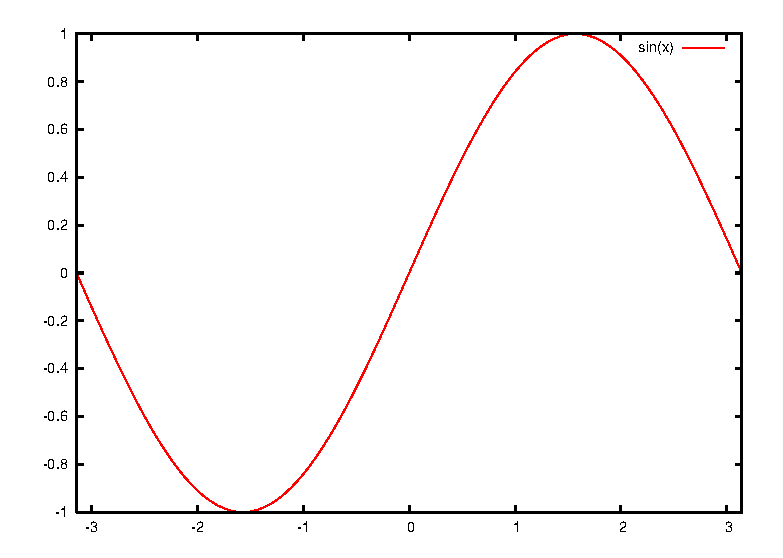
\includegraphics[width=50mm]{sin.eps}\\
これが$\sin x$のグラフです。
\end{verbatim}
\end{screen}
\end{minipage}%
%\manerrarrow\hfill{}
$\Rightarrow$
\begin{minipage}{.45\textwidth}
\begin{shadebox}
幅50mmで貼るには\\
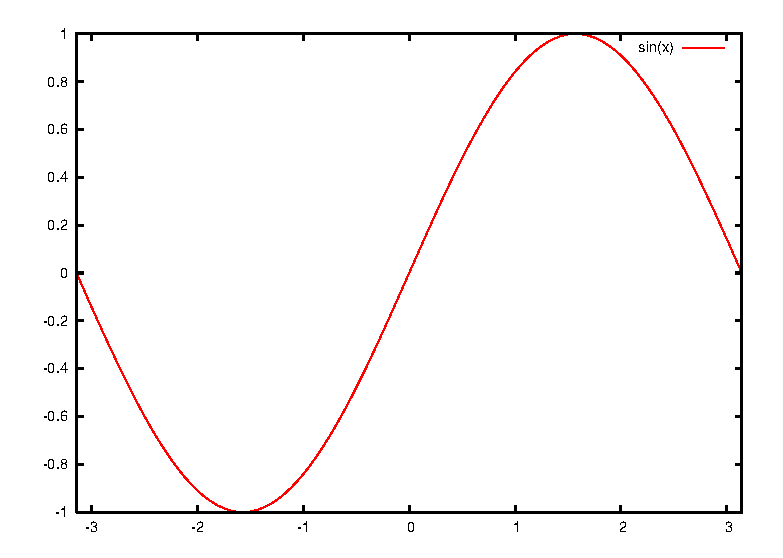
\includegraphics[width=50mm]{sin.eps}\\
これが$\sin x$のグラフです。
\end{shadebox}
\end{minipage}
\vspace*{1mm}\\
\\
\begin{minipage}[c]{.50\textwidth}
\begin{screen}
\small
\begin{verbatim}
高さ20mmで貼るには\\
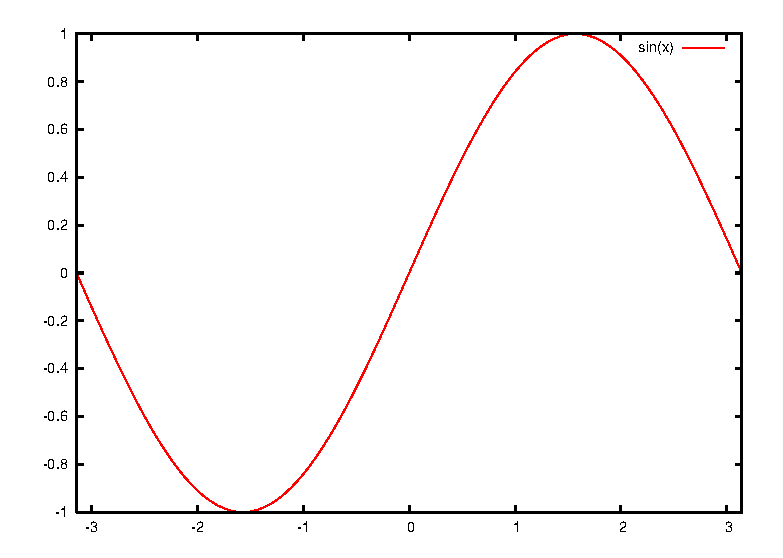
\includegraphics[height=20mm]{sin.eps}\\
これが$\sin x$のグラフです。
\end{verbatim}
\end{screen}
\end{minipage}%
%\manerrarrow\hfill{}
$\Rightarrow$
\begin{minipage}{.45\textwidth}
\begin{shadebox}
高さ20mmで貼るには\\
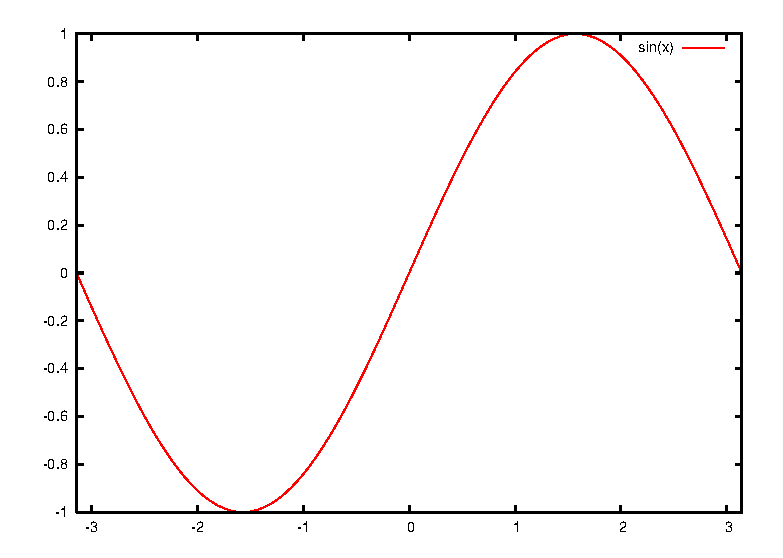
\includegraphics[height=20mm]{sin.eps}\\
これが$\sin x$のグラフです。
\end{shadebox}
\end{minipage}
\vspace*{1mm}\\
\\
\begin{minipage}[c]{.50\textwidth}
\begin{screen}
\small
\begin{verbatim}
縦横比を壊すことも可能です。\\
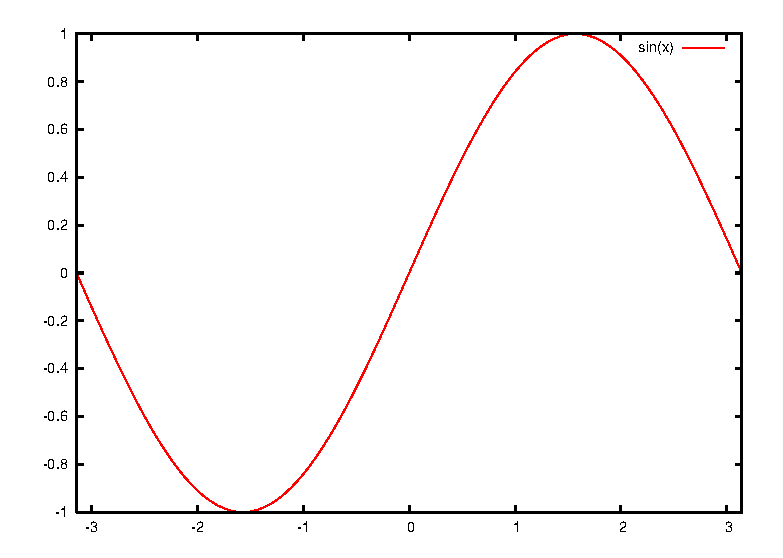
\includegraphics[height=20mm,width=50mm]
{sin.eps}\\
これが$\sin x$のグラフです。
\end{verbatim}
\end{screen}
\end{minipage}%
%\manerrarrow\hfill{}
$\Rightarrow$
\begin{minipage}{.45\textwidth}
\begin{shadebox}
縦横比を壊すことも可能です。\\
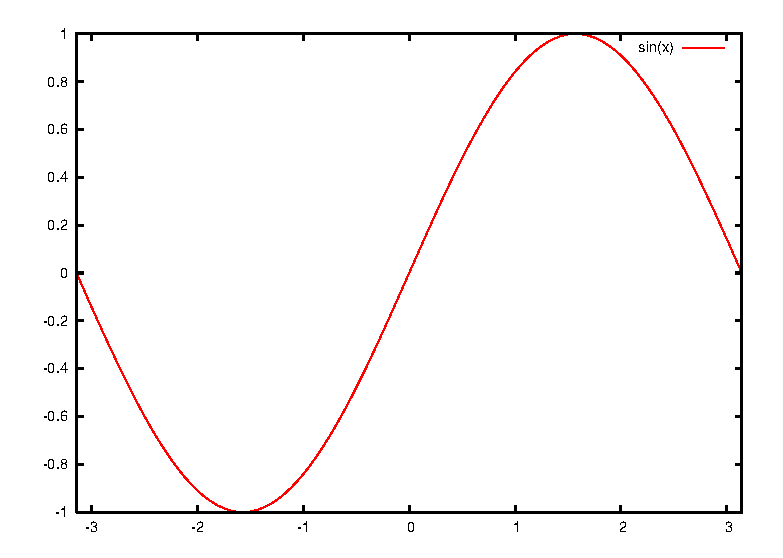
\includegraphics[height=20mm,width=50mm]
{sin.eps}\\
これが$\sin x$のグラフです。
\end{shadebox}
\end{minipage}
\vspace*{1mm}\\
\\
\begin{minipage}[c]{.50\textwidth}
\begin{screen}
\small
\begin{verbatim}
任意の角度だけ図を回転させることも可能です。
ただし角度の単位は\verb+degree+です。\\
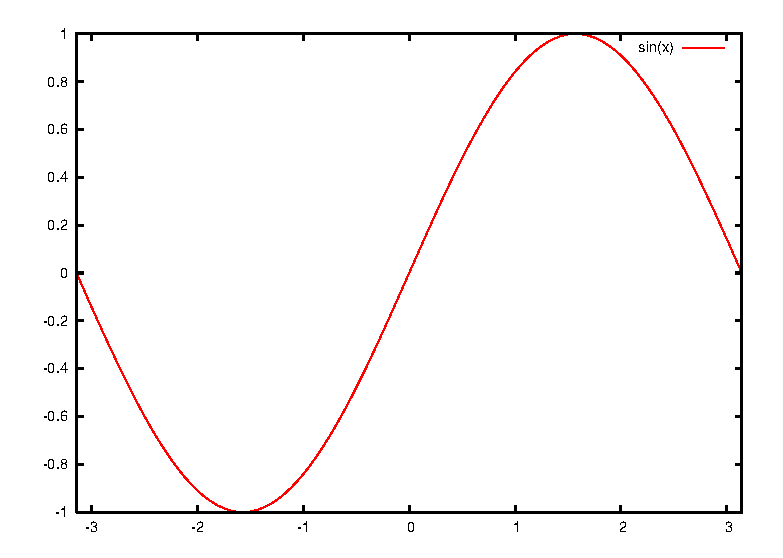
\includegraphics[width=20mm,angle=90.0]
{sin.eps}\\
これが$\sin x$のグラフです。
\end{verbatim}
\end{screen}
\end{minipage}%
%\manerrarrow\hfill{}
$\Rightarrow$
\begin{minipage}{.45\textwidth}
\begin{shadebox}
任意の角度だけ図を回転させることも可能です。
ただし角度の単位は\verb+degree+です。\\
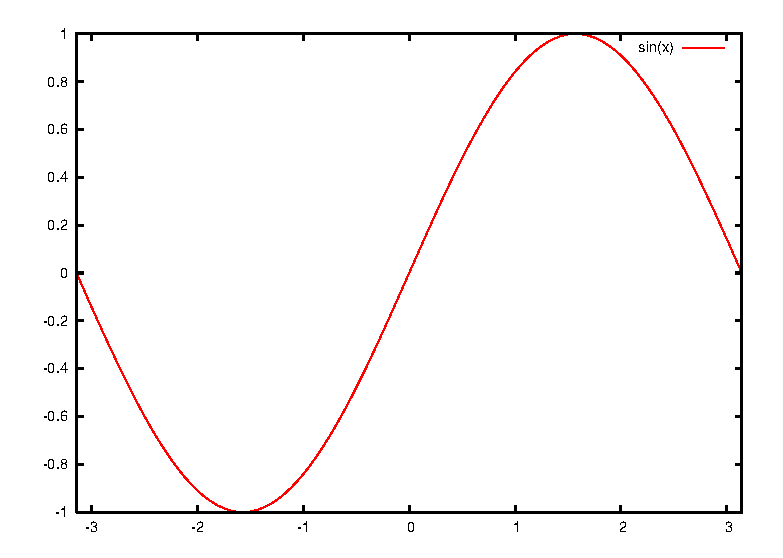
\includegraphics[width=20mm,angle=90.0]
{sin.eps}\\
これが$\sin x$のグラフです。
\end{shadebox}
\end{minipage}
\vspace*{1mm}\\

\subsection{浮動体}
この節の最初に書いたように、図や表の書き方には決まりがあります。これを実
現するために,{\LaTeX}には「浮動体(float)」という概念があります。具体的
には、表を貼り込むときはtable環境で、図を張り込むときはfigure
環境で入れ子にしてやります。こうすることで{\LaTeX}は最適な位置に図や表
を張り込もうとします。図の浮動体の使い方は以下のとおりです。
\begin{screen}
\begin{verbatim}
\begin{figure}[位置指定子]
\includegraphics[設定]{ファイル名}
\caption{図の見出し}
\label{ラベル}
\end{figure}
\end{verbatim}
\end{screen}
一方、表の浮動体の使い方は
\begin{screen}
\begin{verbatim}
\begin{table}[位置指定子]
\caption{表の見出し}
\label{ラベル}
\begin{tabular}
(実際の表本体)
\end{tabular}
\end{table}
\end{verbatim}
\end{screen}
このうち、\verb+\includegraphics+やtabular環境などは
\ref{sub:tabular}節や\ref{sub:image}節で説明したものとまったく
同じです。これを、図ならば\verb+\begin{figure}+と\verb+\end{figure}+で、表
なら\verb+\begin{tabular}+と\verb+\end{tabular}+で囲ってやります。
こうすると、{\LaTeX}はこの図や表のセットを持って移動し、もっとも適切な位
置に出力します。例えばページの下で狭くて入りきらないときは、次のページ
の上のほうに出力しようとするわけです。

ただし、出力位置はある程度はユーザがコントロールすることができます。それが
位置指定子です。位置指定子には表\ref{tab:float}に示すような種類が
あります。
\begin{table}[htbp]
\begin{center}
\caption{浮動体の位置指定子}
\label{tab:float}
\begin{tabular}{cl}
\hline
記号     & 配置する場所           \\
\hline
\verb+h+ & まさにその場所         \\
\verb+t+ & ページの上部           \\
\verb+b+ & ページの下部           \\
\verb+p+ & 新たに別ページをおこす \\
\hline
\end{tabular}
\end{center}
\end{table}
位置指定子を書くことで、図の出力可能位置を指定することができます。
例えば\verb+[htbp]+と書いたりします。何も指定しなければ\verb+[tbp]+
となります。位置指定子は出力可能な場所を指定しているだけなので、htbpを
並べる順番は関係ありません。

\verb+\caption+には図や表のタイトルを記入します。図のタイトルは図の
下、表のタイトルは表の上、という決まりがあるので、図と表では\verb+\caption+
を入力する位置が異なります。

仮に図や表が次のページに旅立っていってしまったとしても、私たちは図や表に
番号が付いているおかげで参照することができます。それが
\verb+\label{ラベル}+の役割です。例えばこのあたりの原稿は次のように書
かれています\footnote{表やグラフを中央揃えにする場合、\verb+\begin{center}+の代わりに\verb+\centering+とする方法もあります。こちらの方が好ましい場合もあります。詳しくは調べてみてください。}。
\begin{screen}
\begin{verbatim}
出力位置は、ある程度はユーザがコントロールすることができます。それが位置指定子です。
位置指定子には表\ref{tab:float}に示すような種類があります。
\begin{table}[htbp]
\begin{center}
\caption{浮動体の位置指定子}
\label{tab:float}
\begin{tabular}{ll}
    (中略)
\end{tabular}
\end{center}
\end{table}
位置指定子を書くことで,…
\end{verbatim}
\end{screen}
\verb+\label{tab:float}+と\verb+\ref{tab:float}+いう組があるのに気づくで
しょうか。図や表に、引用するときの目安になる目印(\emph{ラベル})をつけ
ておき、本文中でそれを\emph{参照}すると、図や表の通し番号が自動で出力さ
れる、というわけです。\verb+\label+と\verb+\ref+は
組になって働くので、中身は\verb+tab:float+でなくても、\verb+hyou+とか何でもかまいません。要は、
\verb+\ref{ラベル名}+という記述があれば、{\LaTeX}は対応する
\verb+\label{ラベル名}+を探しに行くということです。ついでにこの例で
\verb+\caption+の使い方なども観察しておいてください。

これは非常に便利で合理的な機能なのですが、どうも図や表はその位置に出力さ
れて欲しいと思う人が多いようです。しかし、ここで示した方法がレポートや論
文での正しい参照の仕方ですから、気にすることはありません。また、\emph{決して自分で図の番号を振ろうなんて思ってはいけません}。

\subsection{練習}
プロジェクトtex\_exerciseの中に\underline{exercise4.tex}
と\underline{poincare.eps}があります。\underline{exercise4.tex}を開きコンパイルすると図も表も含まれた文書ができるはずです。まずはな
がめてみるのがよいでしょう。その上で、
\begin{itemize}
\item[-] 図のサイズを変えてみる
\item[-] \verb+\label{poincare}+と\verb+\ref{poincare}+の組を他の名前(例えば
	 \verb+\label{chaos}+と\verb+\ref{chaos}+とか)に変えても
	 結果が変わらないことを確かめてみる
\end{itemize}
ということをやってみましょう。\\

%section 8
%%%%%%%%%%%%%%%%%%%%%%%%%%%%%%%%%%%%%%%
%%%%%%%%%%%%%%%%%%%%%%%%%%%%%%%%%%%%%%%

\section{コマンドの編集}
ここまで読んでくれば、{\TeX}を使って一通りの作業ができ、レポートなどの文書
も書けるようになると思います。しかし記号の一つ一つに対してコマンドが割り
振られている、という{\TeX}の特性上どうしても一つの文書を書き上げるまで多
くの文字を打ち込まなければなりません。ただ面倒臭いと言うだけならまだしも、
レポートなどになると偏微分の記号
$\displaystyle \frac{\partial}{\partial t}$
などがしょっちゅうでてきて、これをいちいち
\verb+\frac{\partial}{\partial t}+などと打ち込んでいるのは辟易してきます。
このような場合には自分で偏微分の記号を一発で表示させるコマンドを作ってしまう方が便利です。
このような場合に非常に重宝するのが\verb+\def+コマンドです。
たぶん\verb+define+かなんかを短縮したものでしょう。
さて、プリアンブルに例えば、
\verb+\def\deln#1{\frac{\partial}{\partial {\mbox{$#1$}}}}+
と打ってみましょう。
これはちょっと長めですが、このあとの幸せを考えるとまあ耐えられます。
さてこの一行の意味ですが、\verb+\def+というコマンドで直後の\verb+\deln+と
いうコマンドを定義せよ、と命令しているわけです。\verb+\deln+の直後の
\verb+#1+は引数を入れる欄を作っています。わざわざ真似て新作のコマンドの名前を
\verb+\deln+にする必要はないですが、
ここでは偏微分の``デル''の分子に``微分される関数が何もつきませんよ(nothing)''
のつもりでこの名前にしてます。別に
\verb+\def\riderkick#1+云々でも構いません。こうやった上で微分したい変数を
引数にいれて\\
\begin{minipage}[c]{.50\textwidth}
\begin{screen}
\small
\begin{verbatim}
この様に\\
$\deln{x}$\\
とすれば
\end{verbatim}
\end{screen}
\end{minipage}%
%\manerrarrow\hfill{}
$\Rightarrow$
\begin{minipage}{.45\textwidth}
\begin{shadebox}
この様に\\
$\frac{\partial}{\partial x}$\\
とすれば
\end{shadebox}
\end{minipage}\\
\vspace*{5mm}
ちゃんと偏微分が表示されています。これはほんの一例ですので色々と各自試し
て見てください。微分の記号くらいは充実させておくと便利です。なお
\verb+\def+の代わりに
\verb+\newcommand+でも似たような操作ができるみたいです。興味がある人は調べてみてください。

\pagebreak
%kadai
%%%%%%%%%%%%%%%%%%%%%%%%%%%%%%%%%%%%%%%
%%%%%%%%%%%%%%%%%%%%%%%%%%%%%%%%%%%%%%%

\section{課題:数式の書き方,図の貼り込み}
\underline{/home2/takata2022/homework/homework.pdf}という文書があります。
しかしこの文書には残念ながら適当な図が貼り付けてありません。
本文を{\TeX}で作成し、
先日習ったgnuplotで適切な図を作成し
(どんな図でもいいです、また以前つくったものでも構いません)、貼り付けましょう。
ついでに、
文書の最初に課題名、名前、学籍番号、提出日も入れておきましょう。
空白の大きさ等細かい所まで配布文書をまねる必要はないですが、
図の番号付け等、最低限レポートとして人に見せられる体裁は整えましょう。

余裕がある人は図の下または次ページに何かをつけ加えてみてください(箇条書き等の、課題でまだ使っていないコマンドを使ってみる。図を横に複数枚並べてみる。など)。
\\

文書作成の際には新しいプロジェクトを立ち上げてください(この際\ref{sec:overleaf}で行った設定を忘れずに)。
出来上がったら、pdfファイルとソースファイルをダウンロードし、
slackのダイレクトメッセージで\verb+.zip+ファイルを高田に送ってください。
期限は4月20日(水)12:59(JST)とします。



\pagebreak

%Appendix
%%%%%%%%%%%%%%%%%%%%%%%%%%%%%%%%%%%%%%%
%%%%%%%%%%%%%%%%%%%%%%%%%%%%%%%%%%%%%%%

\appendix


\section{文字コードの設定}
texファイルの文字コードが適切でないと(559のeduではUTF-8でないと)、文字化けを起こしてしまいます。最悪の場合、platexの段階でエラーを起こしてdviファイルが出来上がらないこともあります。ここではその対処法をまとめておきます。

\subsection{Emacsの文字コードの設定}
以下のコマンドは、打った文字をそのままに、保存する文字コードをUTF-8に設定するものです。
\begin{screen}
\keytop{Ctrl}$+$\keytop{x} \keytop{Enter} \keytop{f}
\end{screen}
しかし、この方法ではEmacsのウィンドウを閉じるたびに文字コードがEUC-JPに戻ってしまいます。毎回これを打ち直すのは面倒ですから、設定ファイル\verb+.emacs+を覗きにいきましょう。

Emacsで.emacsを開きましょう。この中から、
\begin{screen}
\begin{verbatim}
;; YaTeX-mode
(setq auto-mode-alist
      (cons (cons "\\.tex$" 'yatex-mode) auto-mode-alist))
(setq dvi2-command "xdvi"
      tex-command "platex"
      dviprint-command-format "dvips %s -o !lpr -Pionia"
      YaTeX-kanji-code 3)
\end{verbatim}
\end{screen}
を見つけてください。この中の、\underline{YaTeX-kanji-code 3}が、YaTeXでEUC-JPを使うように、と設定しています。ここを\underline{YaTeX-kanji-code 4}と書き換えます。
\begin{screen}
\begin{verbatim}
;; YaTeX-mode
(setq auto-mode-alist
      (cons (cons "\\.tex$" 'yatex-mode) auto-mode-alist))
(setq dvi2-command "xdvi"
      tex-command "platex"
      dviprint-command-format "dvips %s -o !lpr -Pionia"
      YaTeX-kanji-code 4)
\end{verbatim}
\end{screen}
これでYaTeXがUTF-8を使ってくれるようになります。

先ほどのコマンドとそっくりですが、
\begin{screen}
\keytop{Ctrl}$+$\keytop{x} \keytop{Enter} \keytop{r}
\end{screen}
というものがあります。これはEmacsでファイルを開いたら文字化けした場合に使います。「UTF-8で書いたはずのものが文字化けした」というときにはこれを使って、ミニバッファに`utf-8'と入力すれば良いです。何か聞かれたら`yes'と答えておきましょう。

興味のある人は、\verb+.emacs+内の、
\begin{screen}
\begin{verbatim}
(set-default-coding-systems    'utf-8)
(set-terminal-coding-system    'utf-8)
(set-keyboard-coding-system    'utf-8)
(set-buffer-file-coding-system 'utf-8)
(set-clipboard-coding-system   'utf-8)
(setq default-enable-multibyte-characters t)
\end{verbatim}
\end{screen}
がどういう意味なのか調べてみてください。

\subsection{ターミナルの文字コードの設定}
既に環境変数についてならっていることと思います。ターミナルの文字コードは、この環境変数で設定できます。

現在の文字コードを確認するには、ターミナルで\underline{echo \$LANG}とします。
'\verb+ja_JP.EUC-JP+'と表示されたらEUC-JP、`\verb+ja_JP.utf8+'と表示されたらUTF-8です。UTF-8にしたければ、ターミナル上で\underline{export LANG=ja\_JP.utf8}とします。しかし、この方法では、変更はターミナルを開いている間のみ有効で、一度ターミナルを閉じると、再びEUC-JPに設定されてしまいます。

さて、ホームディレクトリに\verb+.bashrc+というファイルがありましたね。この中身をのぞくと、下の方に
\begin{screen}
\begin{verbatim}
export LANG=ja_JP.EUC-JP
\end{verbatim}
\end{screen}
という行があると思います。ターミナルの文字コードは環境変数\verb+LANG+によって決められており、\verb+.bashrc+によって現在はEUC-JPに設定されています。そこでこの行の頭に\#をつけてコメントアウトし、直後に一行付け加えて、
\begin{screen}
\begin{verbatim}
#export LANG=ja_JP.EUC-JP
export LANG=ja_JP.utf8
\end{verbatim}
\end{screen}
とすることで、ターミナルを立ち上げるたびにUTF-8に設定されるようになります。今すぐにこの変更を適用するには、\underline{source .bashrc}が必要でしたね。

\pagebreak


\section{執筆支援環境}
これまで見てきたとおり、{\LaTeX}の文書はただ文を入力すればよいのではありません。
これは初学者にとっては非常に疲れることです。EmacsにはYaTeXと呼ばれる素晴らしい執筆支援環境があるので紹介します。

\subsection{EmacsとYaTeX(野鳥)}
興味のある人はホームディレクトリにある
.emacsというファイルを\underline{less .emacs}とかでのぞいてみてください。
そこにEmacsでの{\LaTeX}の設定などが書いてあります。
かなりマニアックですが…。

YaTeXの細かい機能は
\begin{screen}
\begin{verbatim}
http://www.yatex.org/
\end{verbatim}
\end{screen}
からたどれますが、この中から主な機能を抜き出すと次のようになります。
以下、例えば\keytop{SPC}はスペースキーを押すことをあらわします。

\subsubsection{補完入力}
\begin{description}
 \item[begin型補完]
   \keytop{Ctrl}$+$\keytop{C} \keytop{Ctrl}$+$\keytop{B} \keytop{SPC}と入力すると、ミニバッファで
   \begin{screen}
     {\tt Begin environment(default document):}
   \end{screen}
   とか聞いてきます。この状態でそのまま\keytop{Enter}を入力すれ
   ば、
   \begin{screen}
\begin{verbatim}
\begin{document}

\end{document}
\end{verbatim}
   \end{screen}
   のような\verb+\begin{環境名} +$\cdots$
   \verb+\end{環境名}+の組み合わせが出てきま
   す。もし、自分が入力したいのはほかの環境名だぜ、というときは、
   その環境の名前({\tt equation}とか)を入力して\keytop{Enter}
   すればよいのですが、たいていは頭文字({\tt equation}なら
   \keytop{E})と\keytop{Tab}で補完してくれます。

 \item[section型補完]
   \keytop{Ctrl}$+$\keytop{C} \keytop{Ctrl}$+$\keytop{S} と入力すると
   \begin{screen}
     {\tt (C-v for view-section) ???\{\}(default documentclass):}
   \end{screen}
   とか聞いてくるので、以下同じ。

 \item[large型補完]
   \keytop{Ctrl}$+$\keytop{C} \keytop{Ctrl}$+$\keytop{L}と入力すると,
   \begin{screen}
     {\tt \{??? \}(default large):}
   \end{screen}
   とか聞いてきます。もう予想はつくと思いますが、ここで
   \keytop{Enter}すれば、\verb+{+\verb+\large+ \verb+}+となって、
   カーソルは``\verb+{+''と``\verb+}+''の間に移ります。

 \item[随時補完] このほかにも、\verb+\bigskip+のような長いコマンドを入力す
   るときは、最初の数文字と\keytop{Ctrl}$+$\keytop{C}
   \keytop{SPC}で補ってくれます。自分の希望するものでなければ
   \keytop{Tab}を入力すれば一覧が出ます。

 \item[ギリシア文字,数式記号補完]
	    ギリシア文字や数式記号も一発で補完してくれます。ギリシア文字
	    を打ちたかったら、数式環境の中で\keytop{:}\keytop{頭のアルファ
	      ベット}を入力すればよく、数式記号は\keytop{;}に続いて割り当
	    てられてキーを打てばいけます。どのキーが対応するかはググって
	    みましょう。
            例えば$\displaystyle \frac{\partial \alpha}{\partial\beta}$も\\
	    \verb+\frac{\partial \alpha}{\partial\beta}+\\
            なんていちいち入力せずに\\
	    \keytop{;} \keytop{f} \keytop{Enter}, \keytop{;} \keytop{6}
	    \keytop{Enter}, \keytop{:} \keytop{a} \keytop{Enter},
	    \keytop{Enter}, \keytop{;} \keytop{6} \keytop{Enter},
	    \keytop{:} \keytop{b} \keytop{Enter}\\
	    となる訳です。慣れると格段にスピードが上がります。

\end{description}

\subsubsection{おまかせ改行}
itemize,enumerate,description環境の中では、改行した
ら次の行の頭には\verb+\item+とか\verb+\item[*]+とか入力することが多いわけで
す。こんなときは\keytop{Esc}$+$\keytop{Enter}\footnote{これでうまくいかない場合は、\keytop{Alt}$+$\keytop{Enter}}で勝手に\verb+\item+を補って
くれます。

\subsubsection{プロセス起動}
{\LaTeX}のソースを編集中、\keytop{Ctrl}$+$\keytop{C} \keytop{Ctrl}$+$\keytop{T}と入力すると、ミニバッファに
\begin{screen}
\begin{verbatim}
J)latex R)egion E)nv B)ibtex mk(I)dx latex+p(D)f K)ill P)review V)iewErr L)pr
\end{verbatim}
\end{screen}
のように表示されます。この説明に従って、例えば\keytop{J}と入力すれば{\LaTeX}のタイプセットが始まりますし、\keytop{P}とすればxdviが起動します。極めつけに\keytop{D}と入力すると、タイプセットした上でpdfまで作ってくれます。

\subsection{WindowsやMax OS XでEmacs$+$YaTeX}
Windowsな方のために、GNU Emacsによく似たxyzzyというテキストエディタがあ
ります。これにKaTeX(
$\leftarrow$かてふ)というメジャーモードを重ねると、Emacs$+$YaTeX
とほぼ同等の扱いができるようになります。詳しくは
\begin{screen}
 http://www.jsdlab.co.jp/\~kamei/\\
 http://osuneko.at.infoseek.co.jp/xyzzy/xyzzy.html
\end{screen}
あたりからどうぞ。

Mac OS XはそもそもUNIX系OSなので、Emacsは比較的簡単にインストールできます。もちろんCygwinやMSYS2などのUNIX仮想環境を入れれば、Windows上でも本家GNU Emacsを動かすことができます。

\subsection{{\LaTeX}の統合執筆環境}
Emacs$+$YaTeXは、必要十分な機能が揃っていて、何よりもEmacsの操作に長けた人には最適な執筆支援環境です。一方で{\LaTeX}に特化したGUIの統合開発(執筆)環境\footnote{統合開発環境とは、プログラミングに必要なコンパイラやテキストエディタ、プレビューアをGUI(グラフィカルユーザインターフェース)でまとめたソフトウェア環境のことです。例えば、XcodeやVisual Studio,Eclipseなどが有名です。}もたくさん存在し、かなり普及しています。気になる人は調べてみると良いでしょう。統合執筆環境とEmacs$+$YaTeXの大きな違いは、マウス操作でコマンドを選択できる点と、見た目が現代的なことです。ソフトごとに特色があり好みが分かれますが、最近はTeXStudioやLyxなどが流行っているようです。Lyxに至っては、Wordのようにリアルタイムに数式や文章構造の視覚的フィードバックを得ながら{\LaTeX}文書を書くことができます。

\end{document}

